% ============================================
% ПРИЛОЖЕНИЯ
% ============================================

% ----- ПРИЛОЖЕНИЕ А -----
\appsection{Справка о прохождении проверки в системе <<Антиплагиат>>}
\label{app:antiplagiat}

\begin{figure}[H]
	\centering
	\includegraphics[width=0.9\textwidth]{docs/antiplagiarism.pdf}
	\caption{Справка о результатах проверки текста ВКР в системе <<Антиплагиат.ВУЗ>>}
	\label{fig:antiplagiat_report}
\end{figure}

% ----- ПРИЛОЖЕНИЕ Б -----
\appsection{Электронная презентация для предзащиты ВКР}
\label{app:presentation}

В настоящем приложении приведены все основные слайды электронной презентации,
использованной при выступлении на процедуре предзащиты ВКР. Доработка
презентации к итоговой защите проводится по комментариям научного
руководителя.

\begin{figure}[H]
	\centering
	
\includegraphics[width=1\textwidth]{docs/ВКР предзащита 2026_01.jpg}
	\caption{Титульный слайд презентации}
	\label{fig:slide_01}
\end{figure}

\begin{figure}[H]
	\centering
	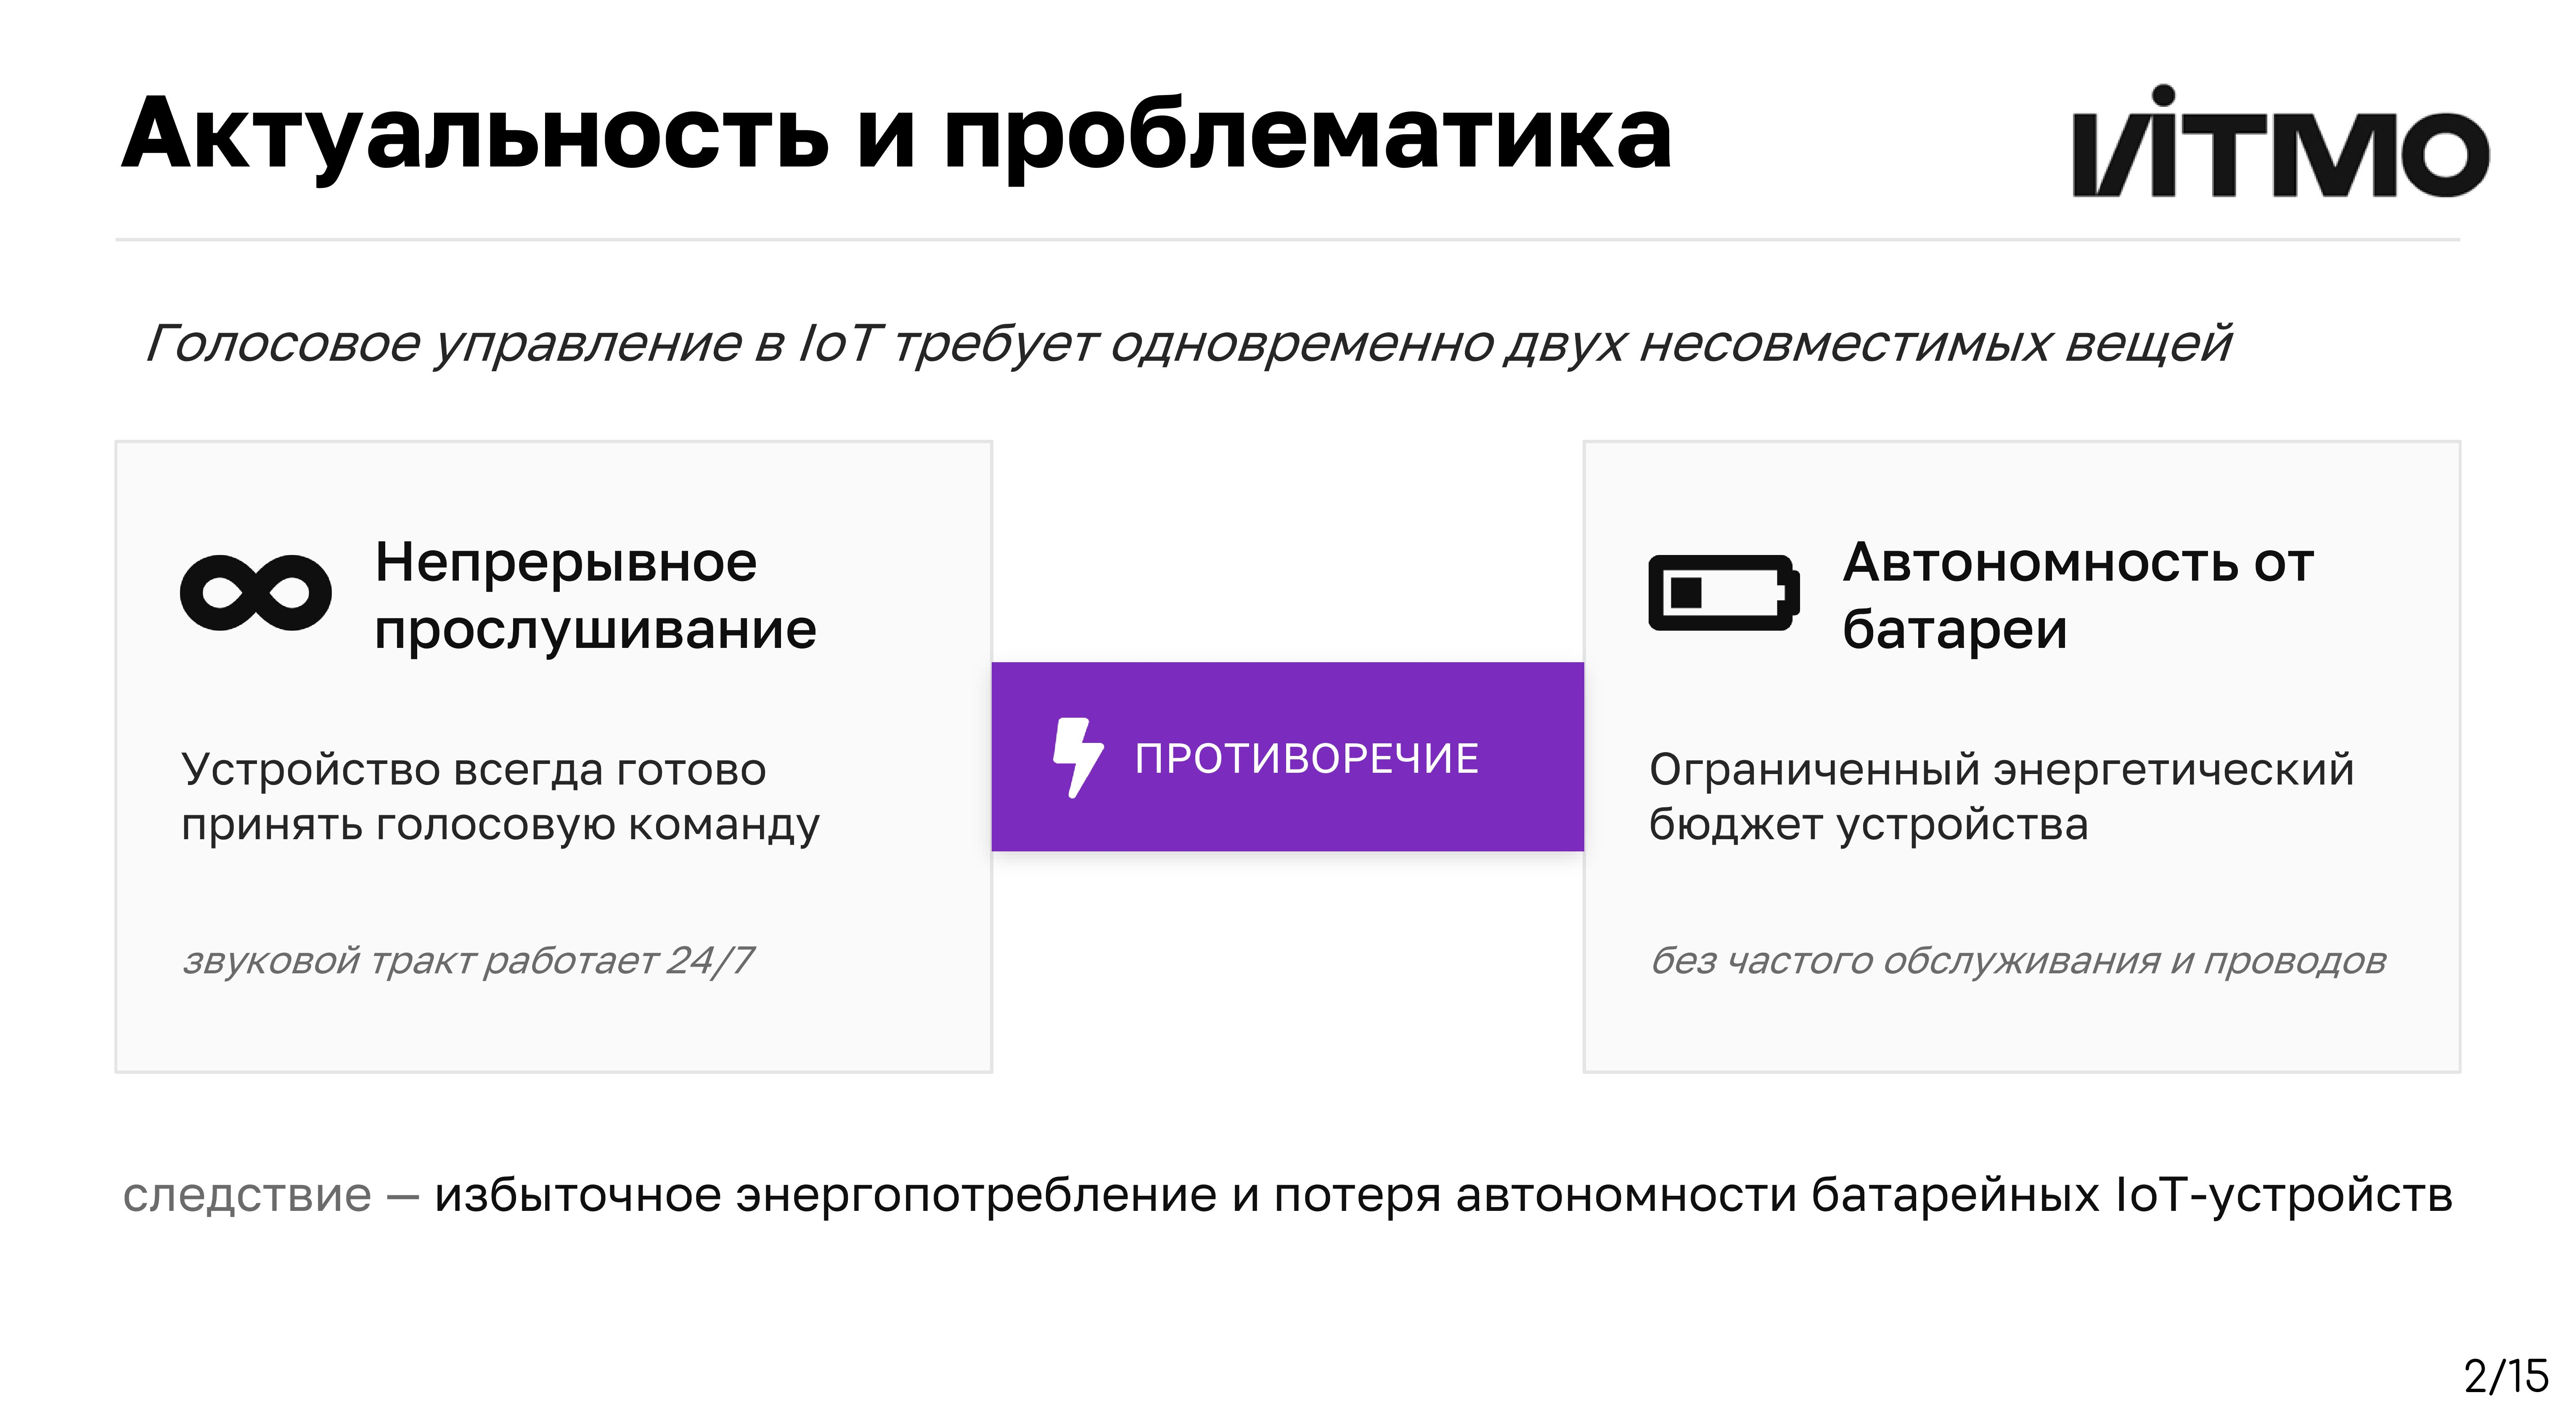
\includegraphics[width=1\textwidth]{docs/ВКР предзащита 2026_02.jpg}
	\caption{Слайд <<Актуальность и проблематика>>}
	\label{fig:slide_02}
\end{figure}

\begin{figure}[H]
	\centering
	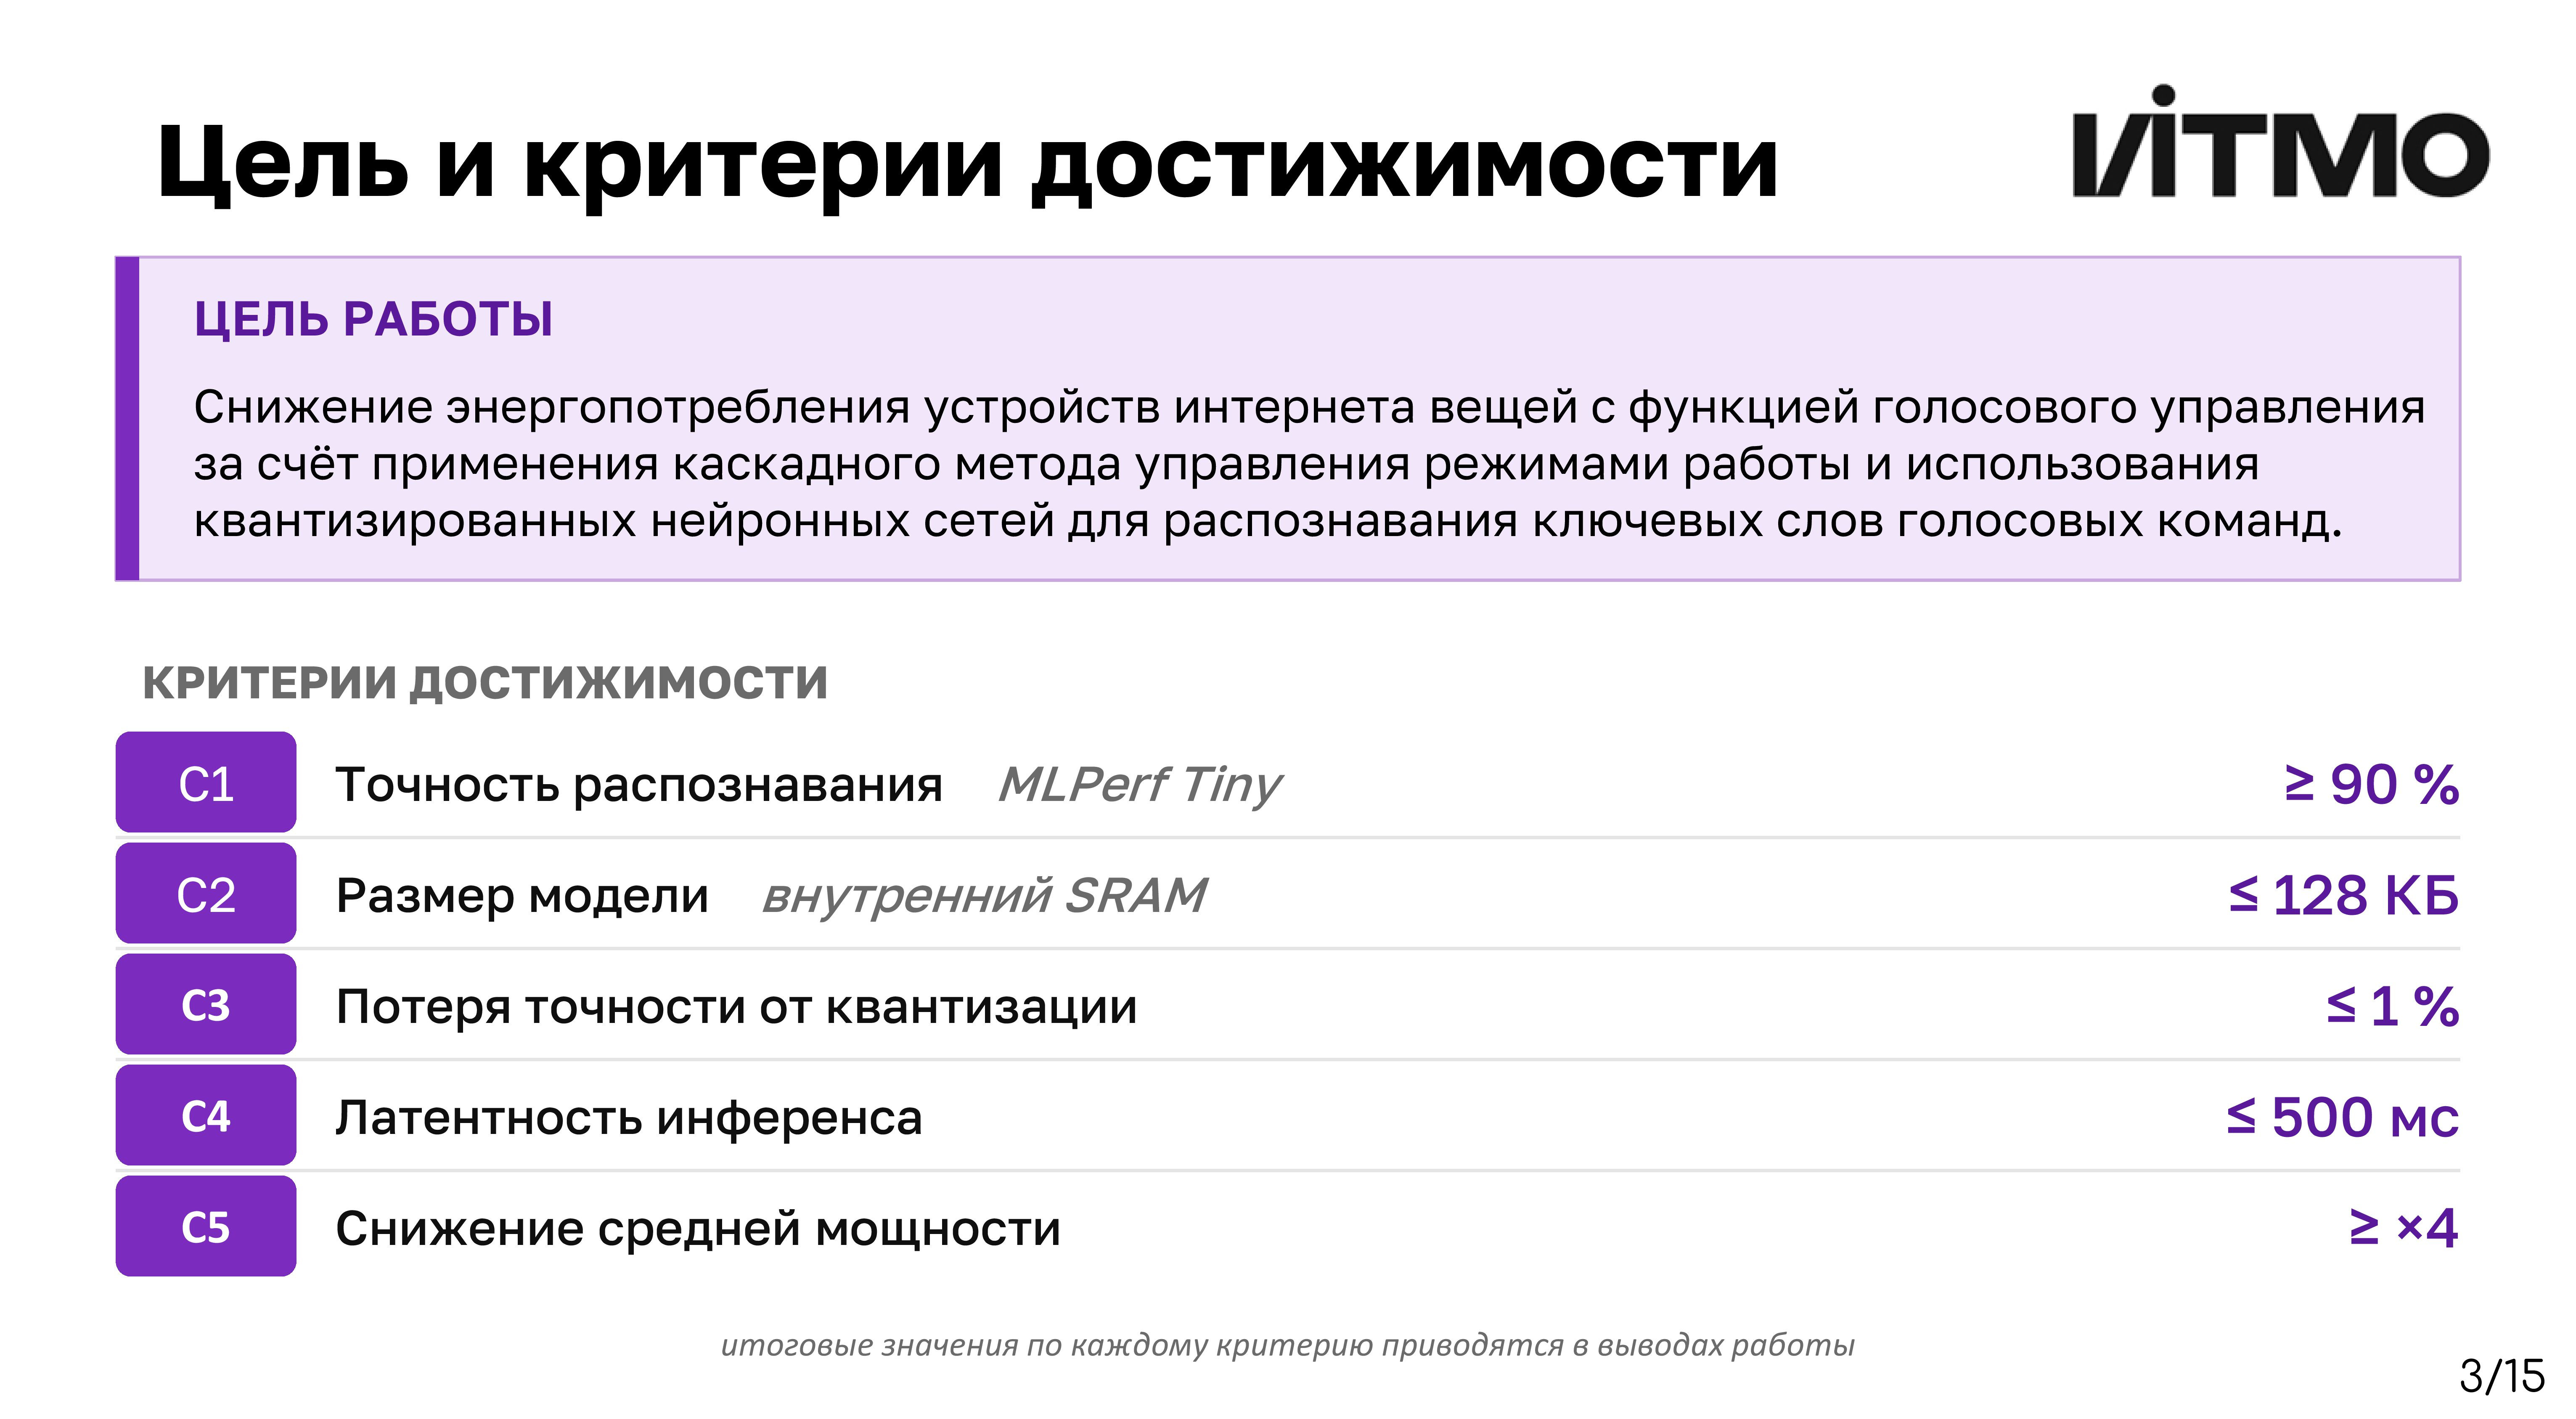
\includegraphics[width=1\textwidth]{docs/ВКР предзащита 2026_03.jpg}
	\caption{Слайд <<Цели и критерии достижимости>>}
	\label{fig:slide_03}
\end{figure}

\begin{figure}[H]
	\centering
	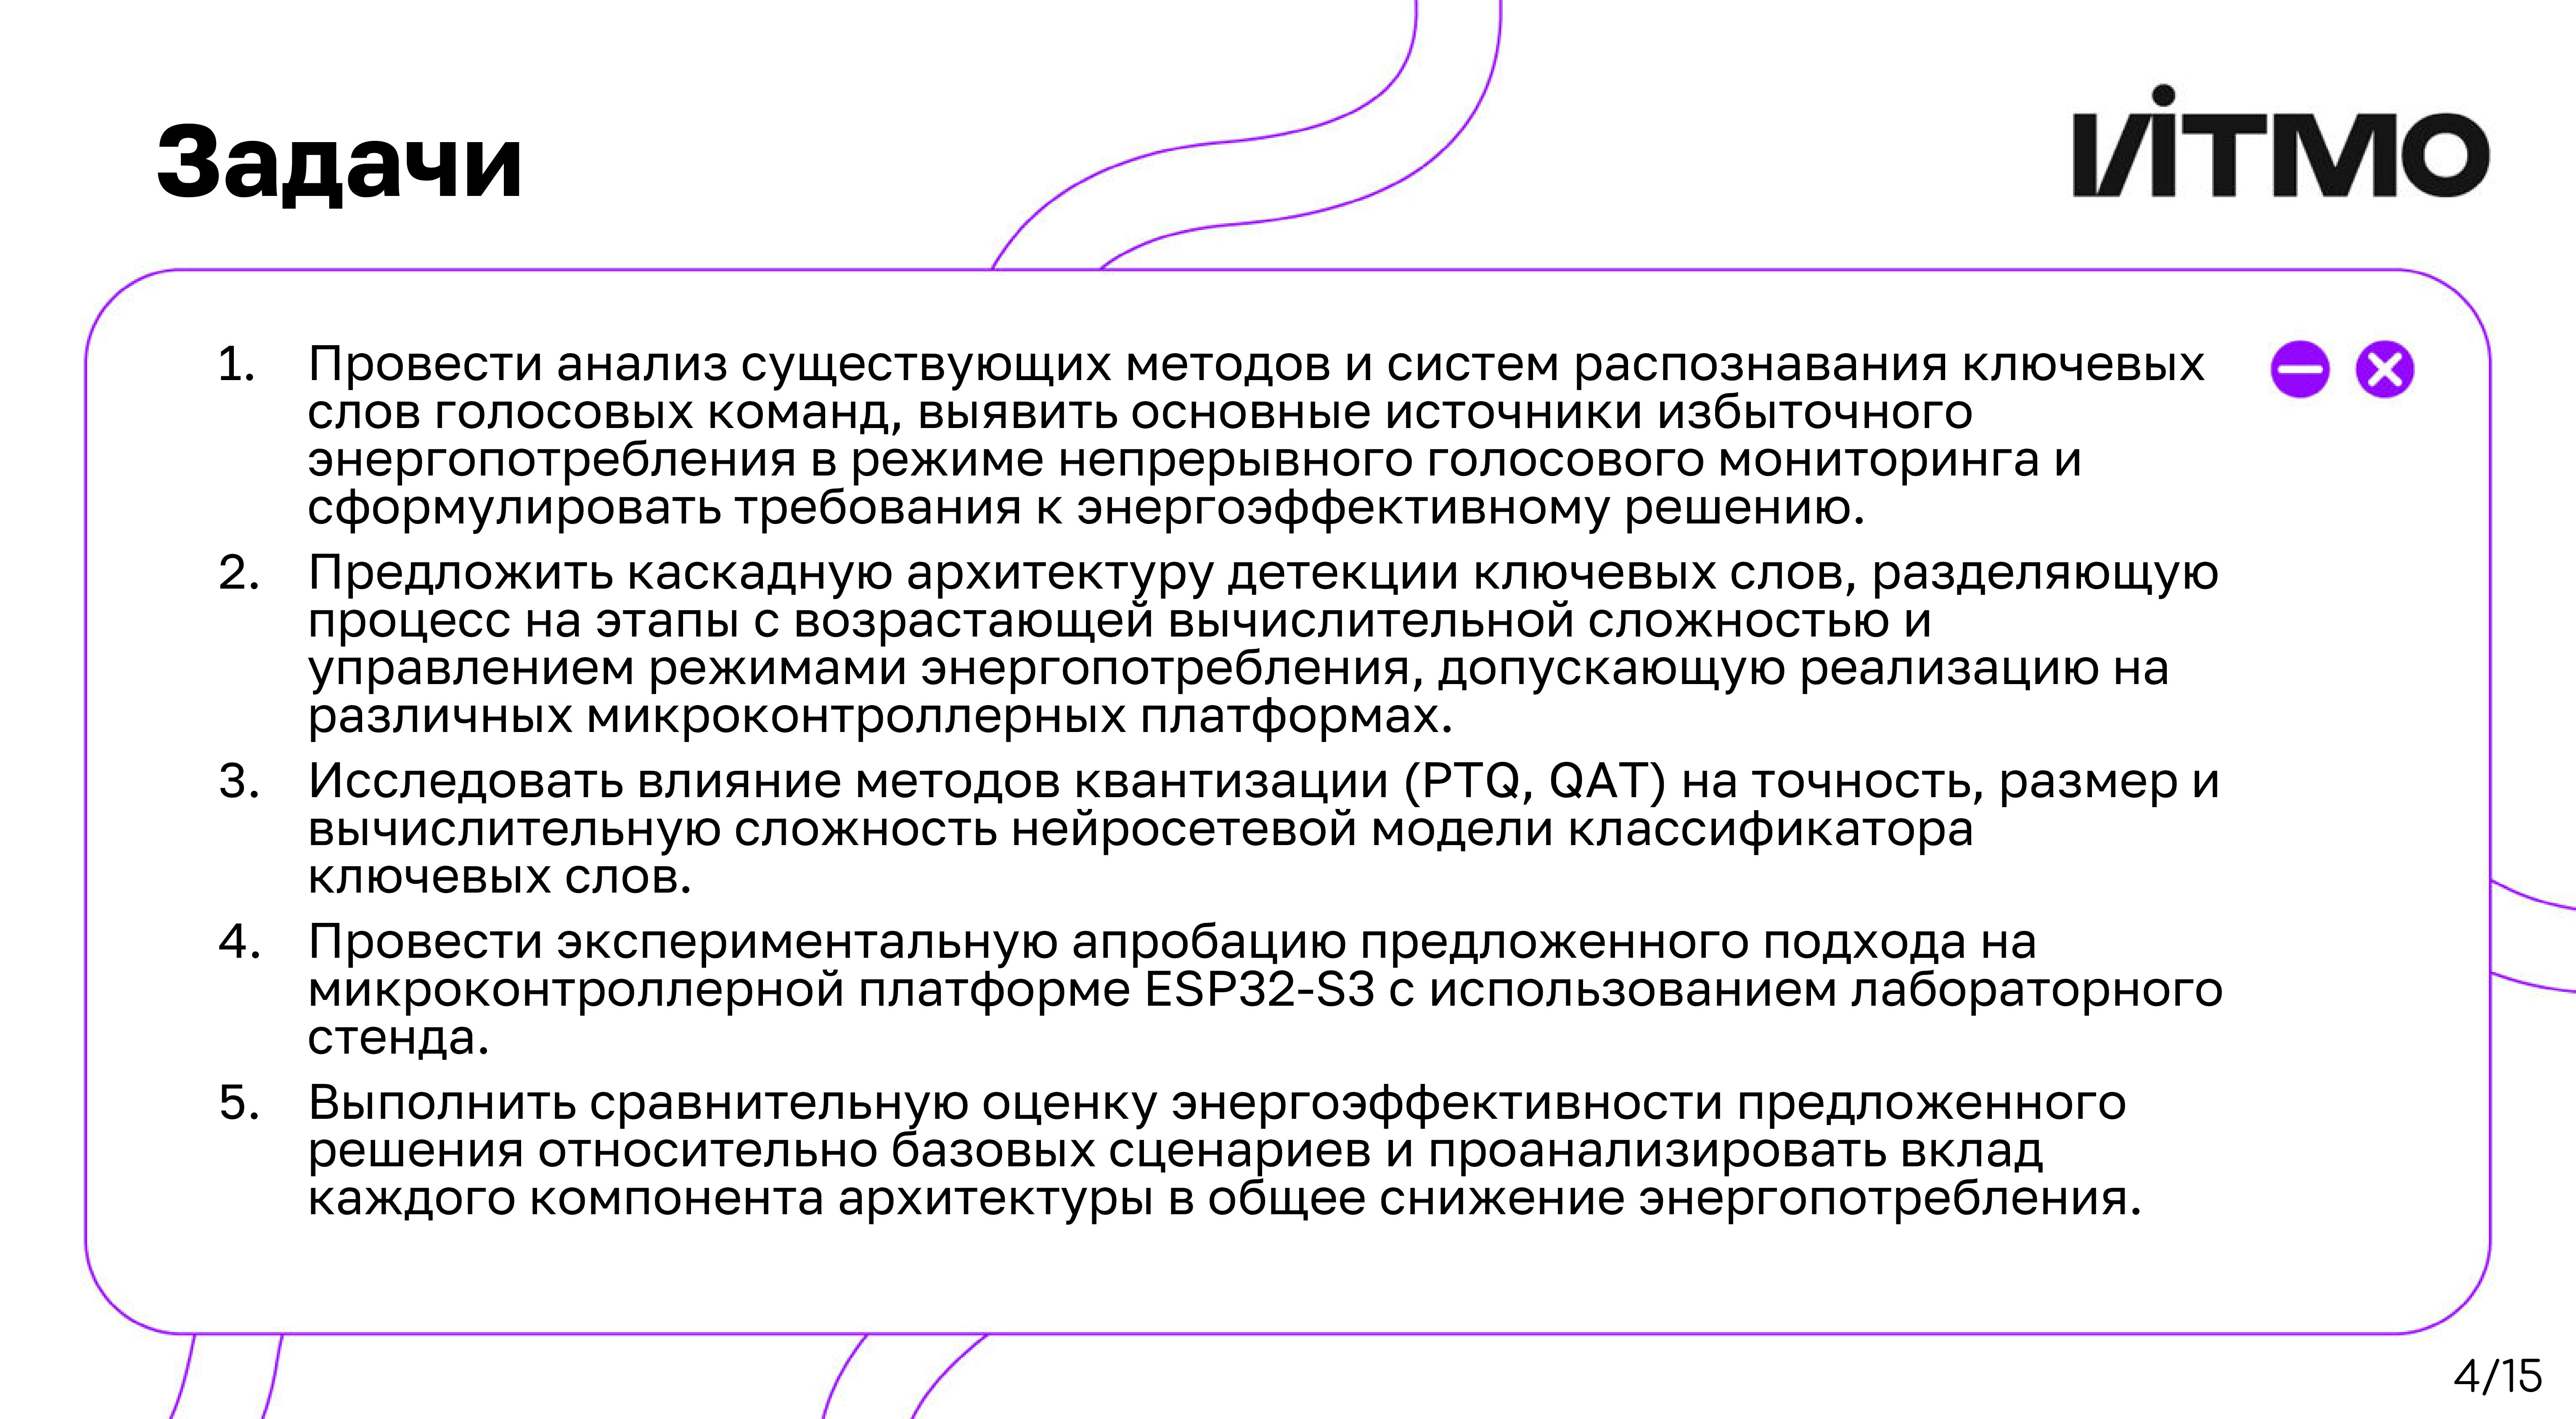
\includegraphics[width=1\textwidth]{docs/ВКР предзащита 2026_04.jpg}
	\caption{Слайд <<Задачи>>}
	\label{fig:slide_04}
\end{figure}

\begin{figure}[H]
	\centering
	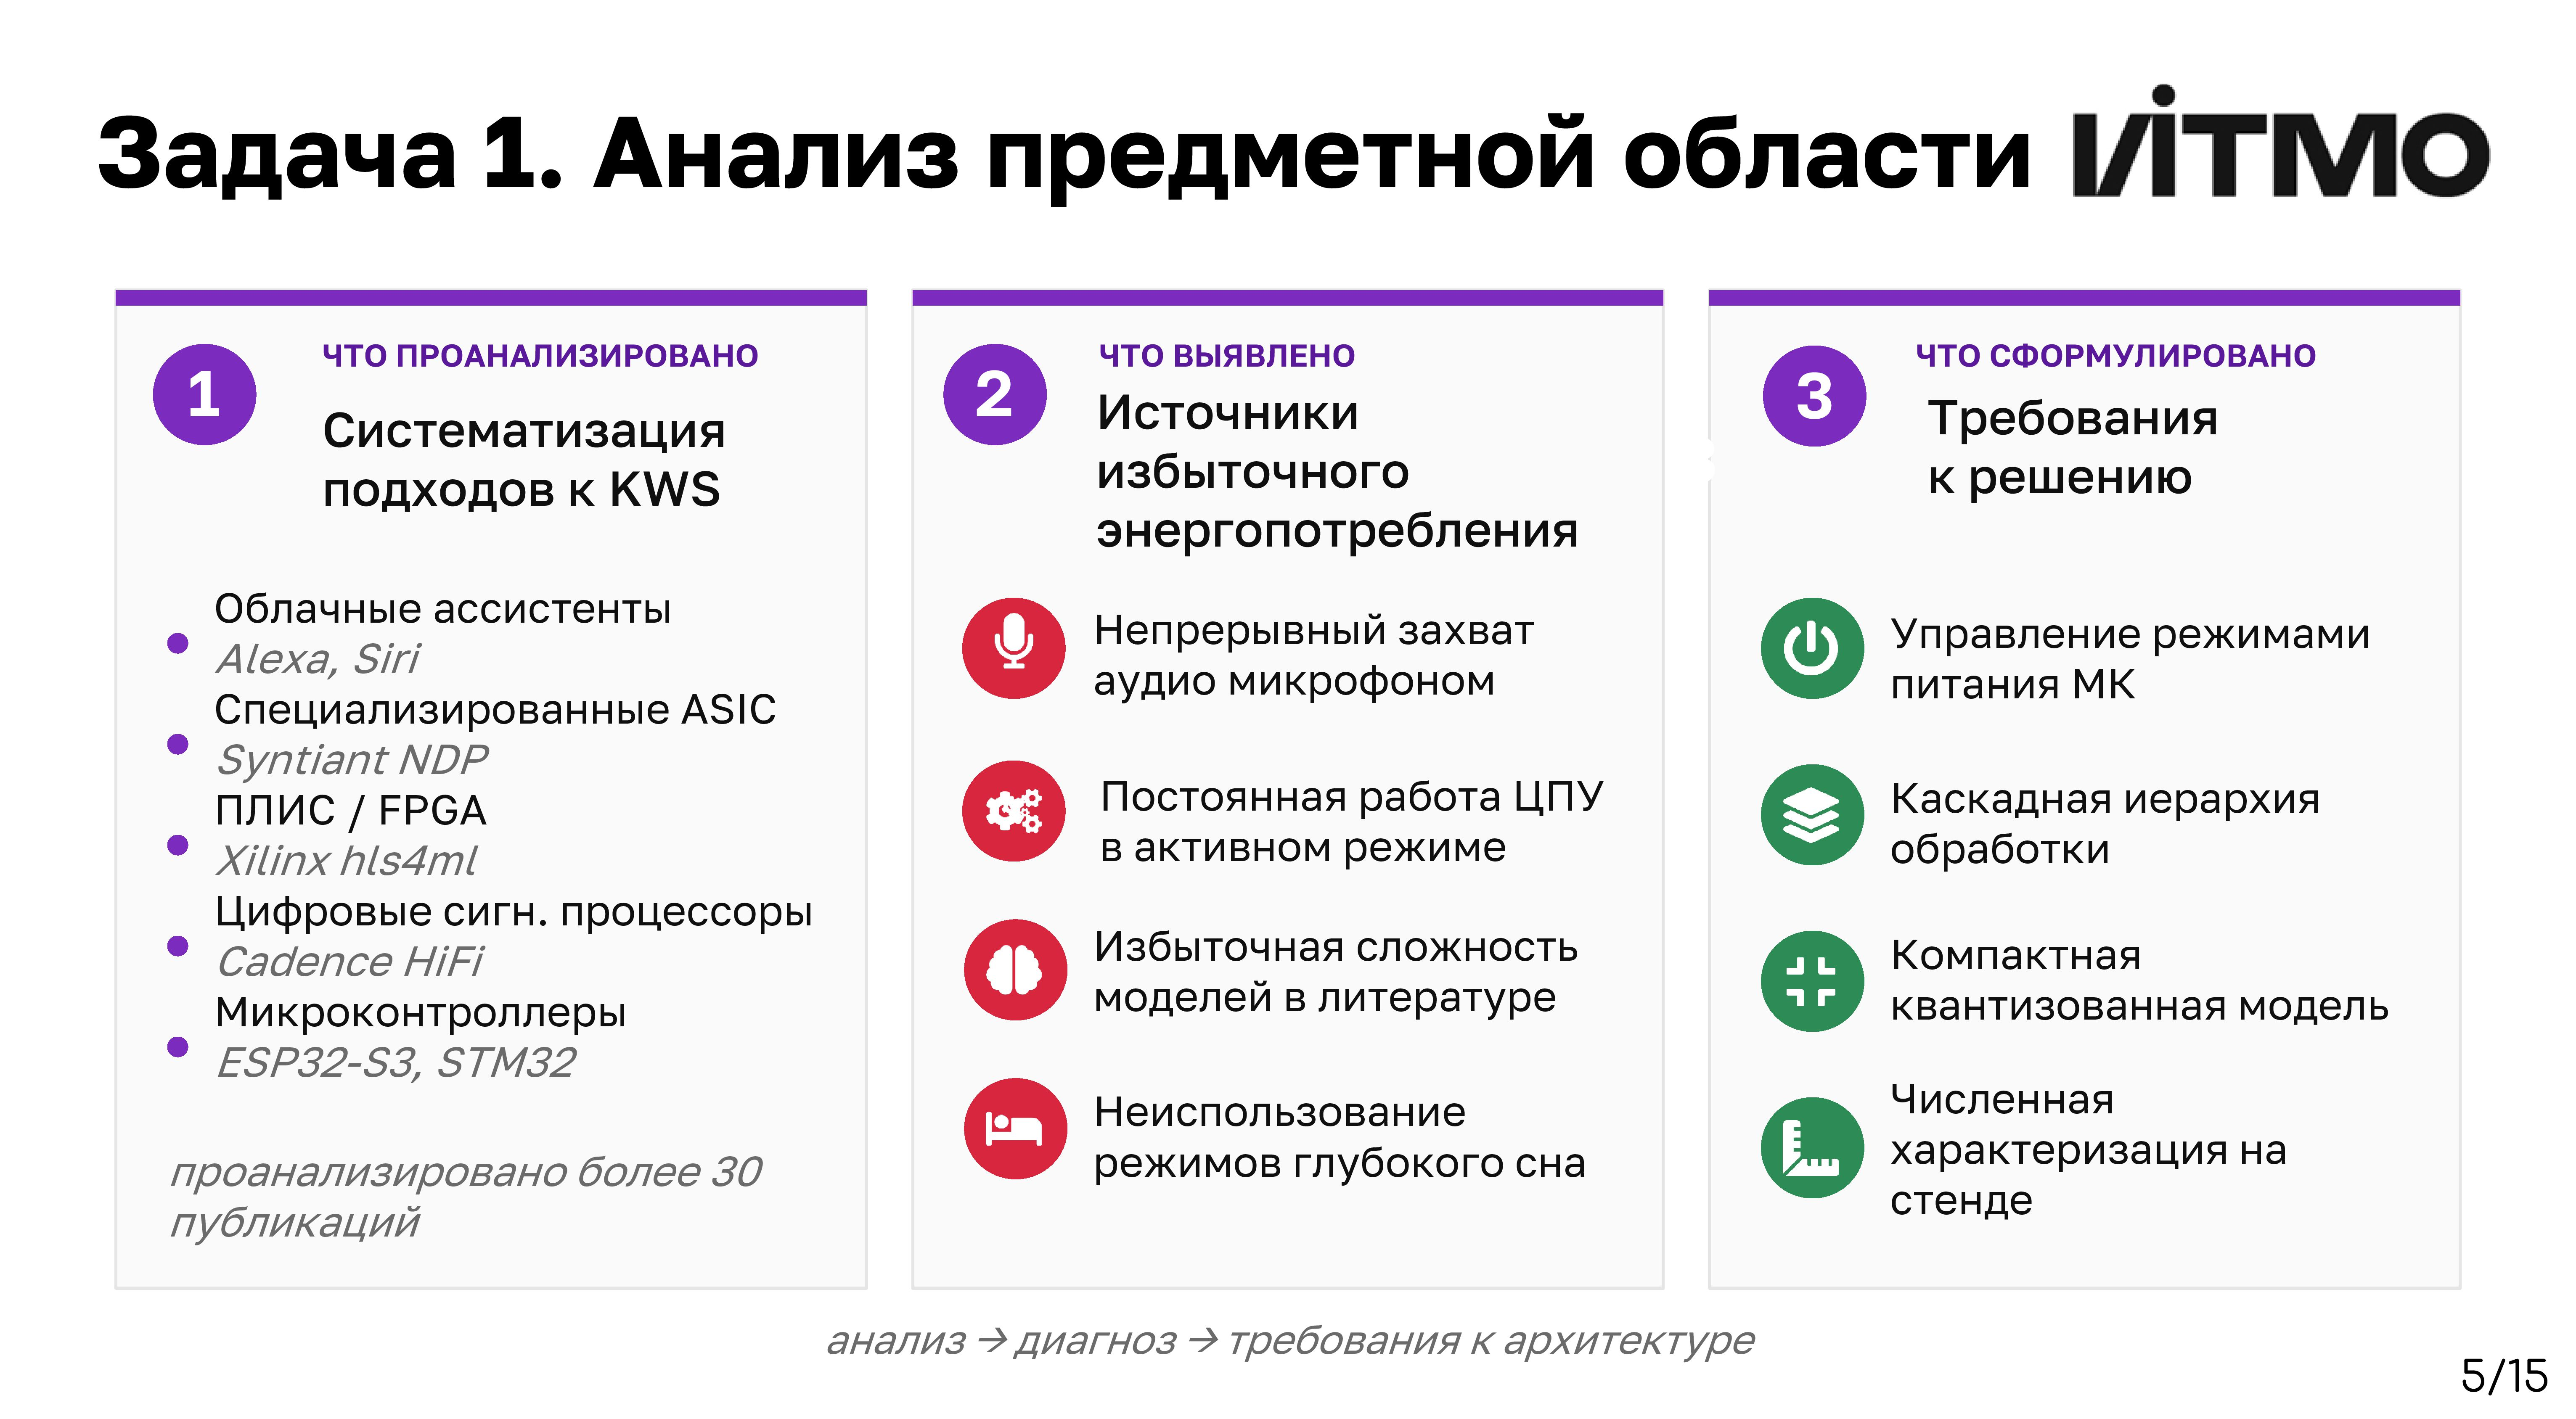
\includegraphics[width=1\textwidth]{docs/ВКР предзащита 2026_05.jpg}
	\caption{Слайд с обзором и анализом предметной области}
	\label{fig:slide_05}
\end{figure}

\begin{figure}[H]
	\centering
	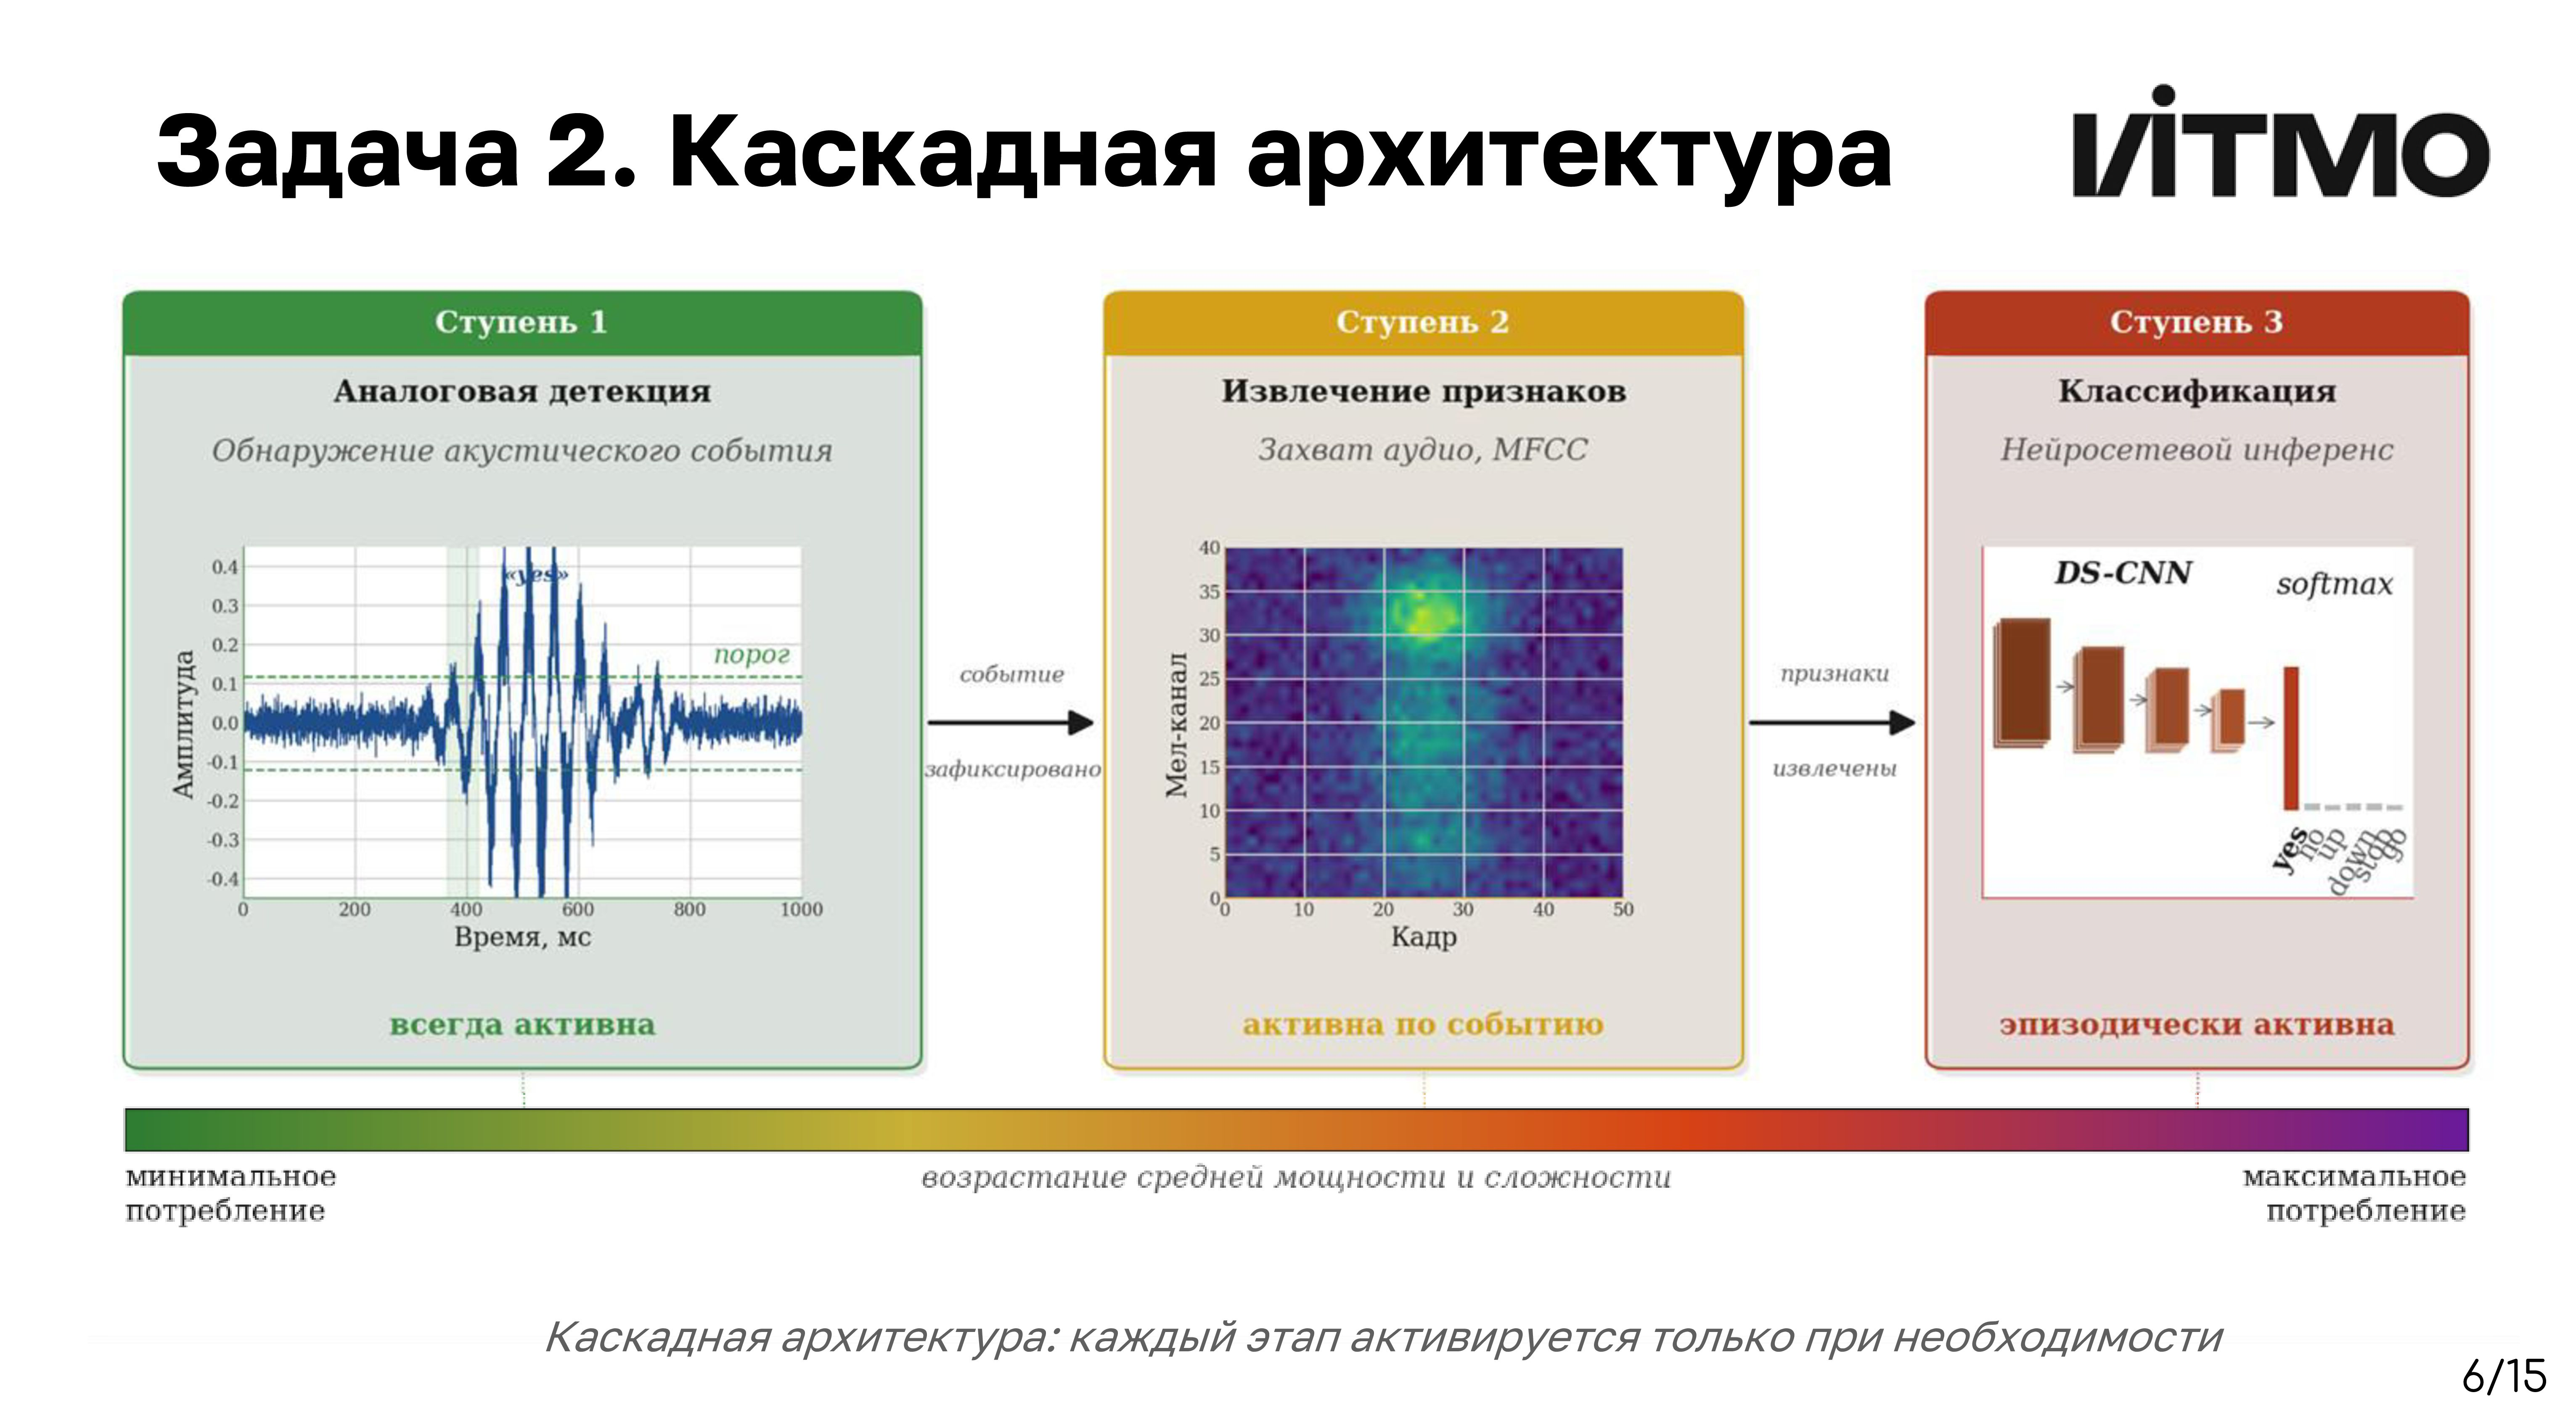
\includegraphics[width=1\textwidth]{docs/ВКР предзащита 2026_06.jpg}
	\caption{Слайд с обзором каскадной архитектуры}
	\label{fig:slide_06}
\end{figure}

\begin{figure}[H]
	\centering
	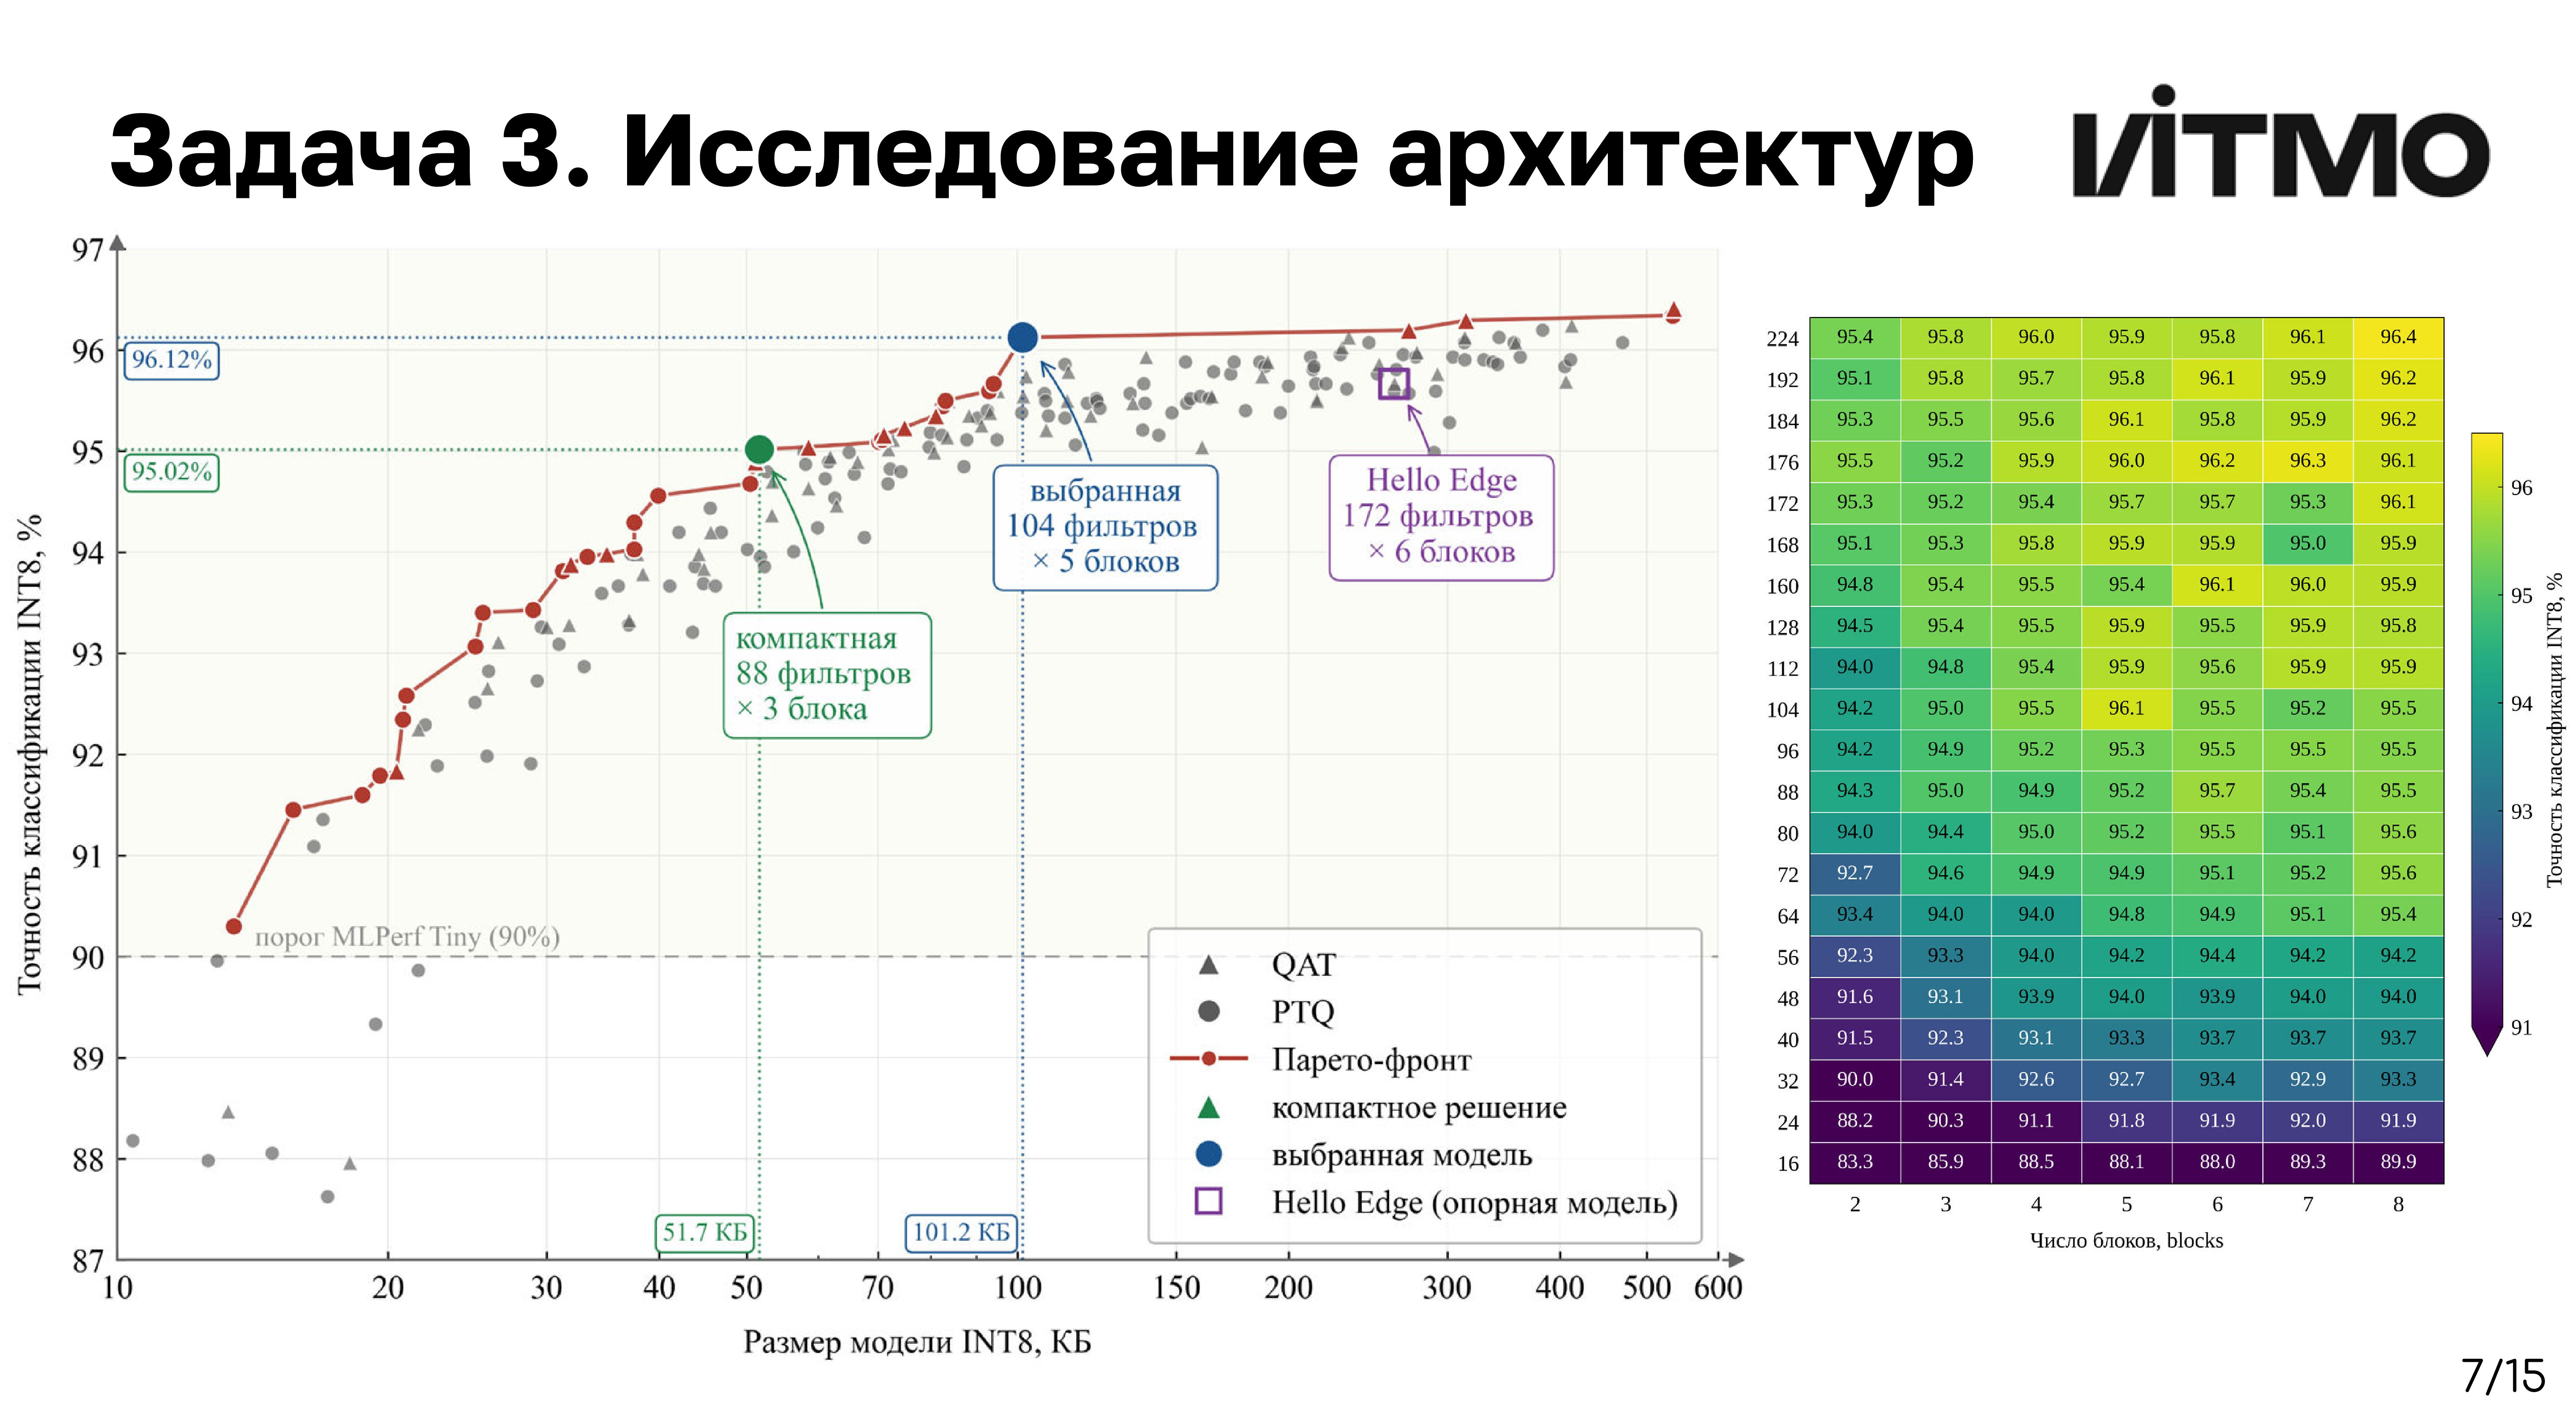
\includegraphics[width=1\textwidth]{docs/ВКР предзащита 2026_07.jpg}
	\caption{Слайд <<Исследования архитектур>>}
	\label{fig:slide_07}
\end{figure}

\begin{figure}[H]
	\centering
	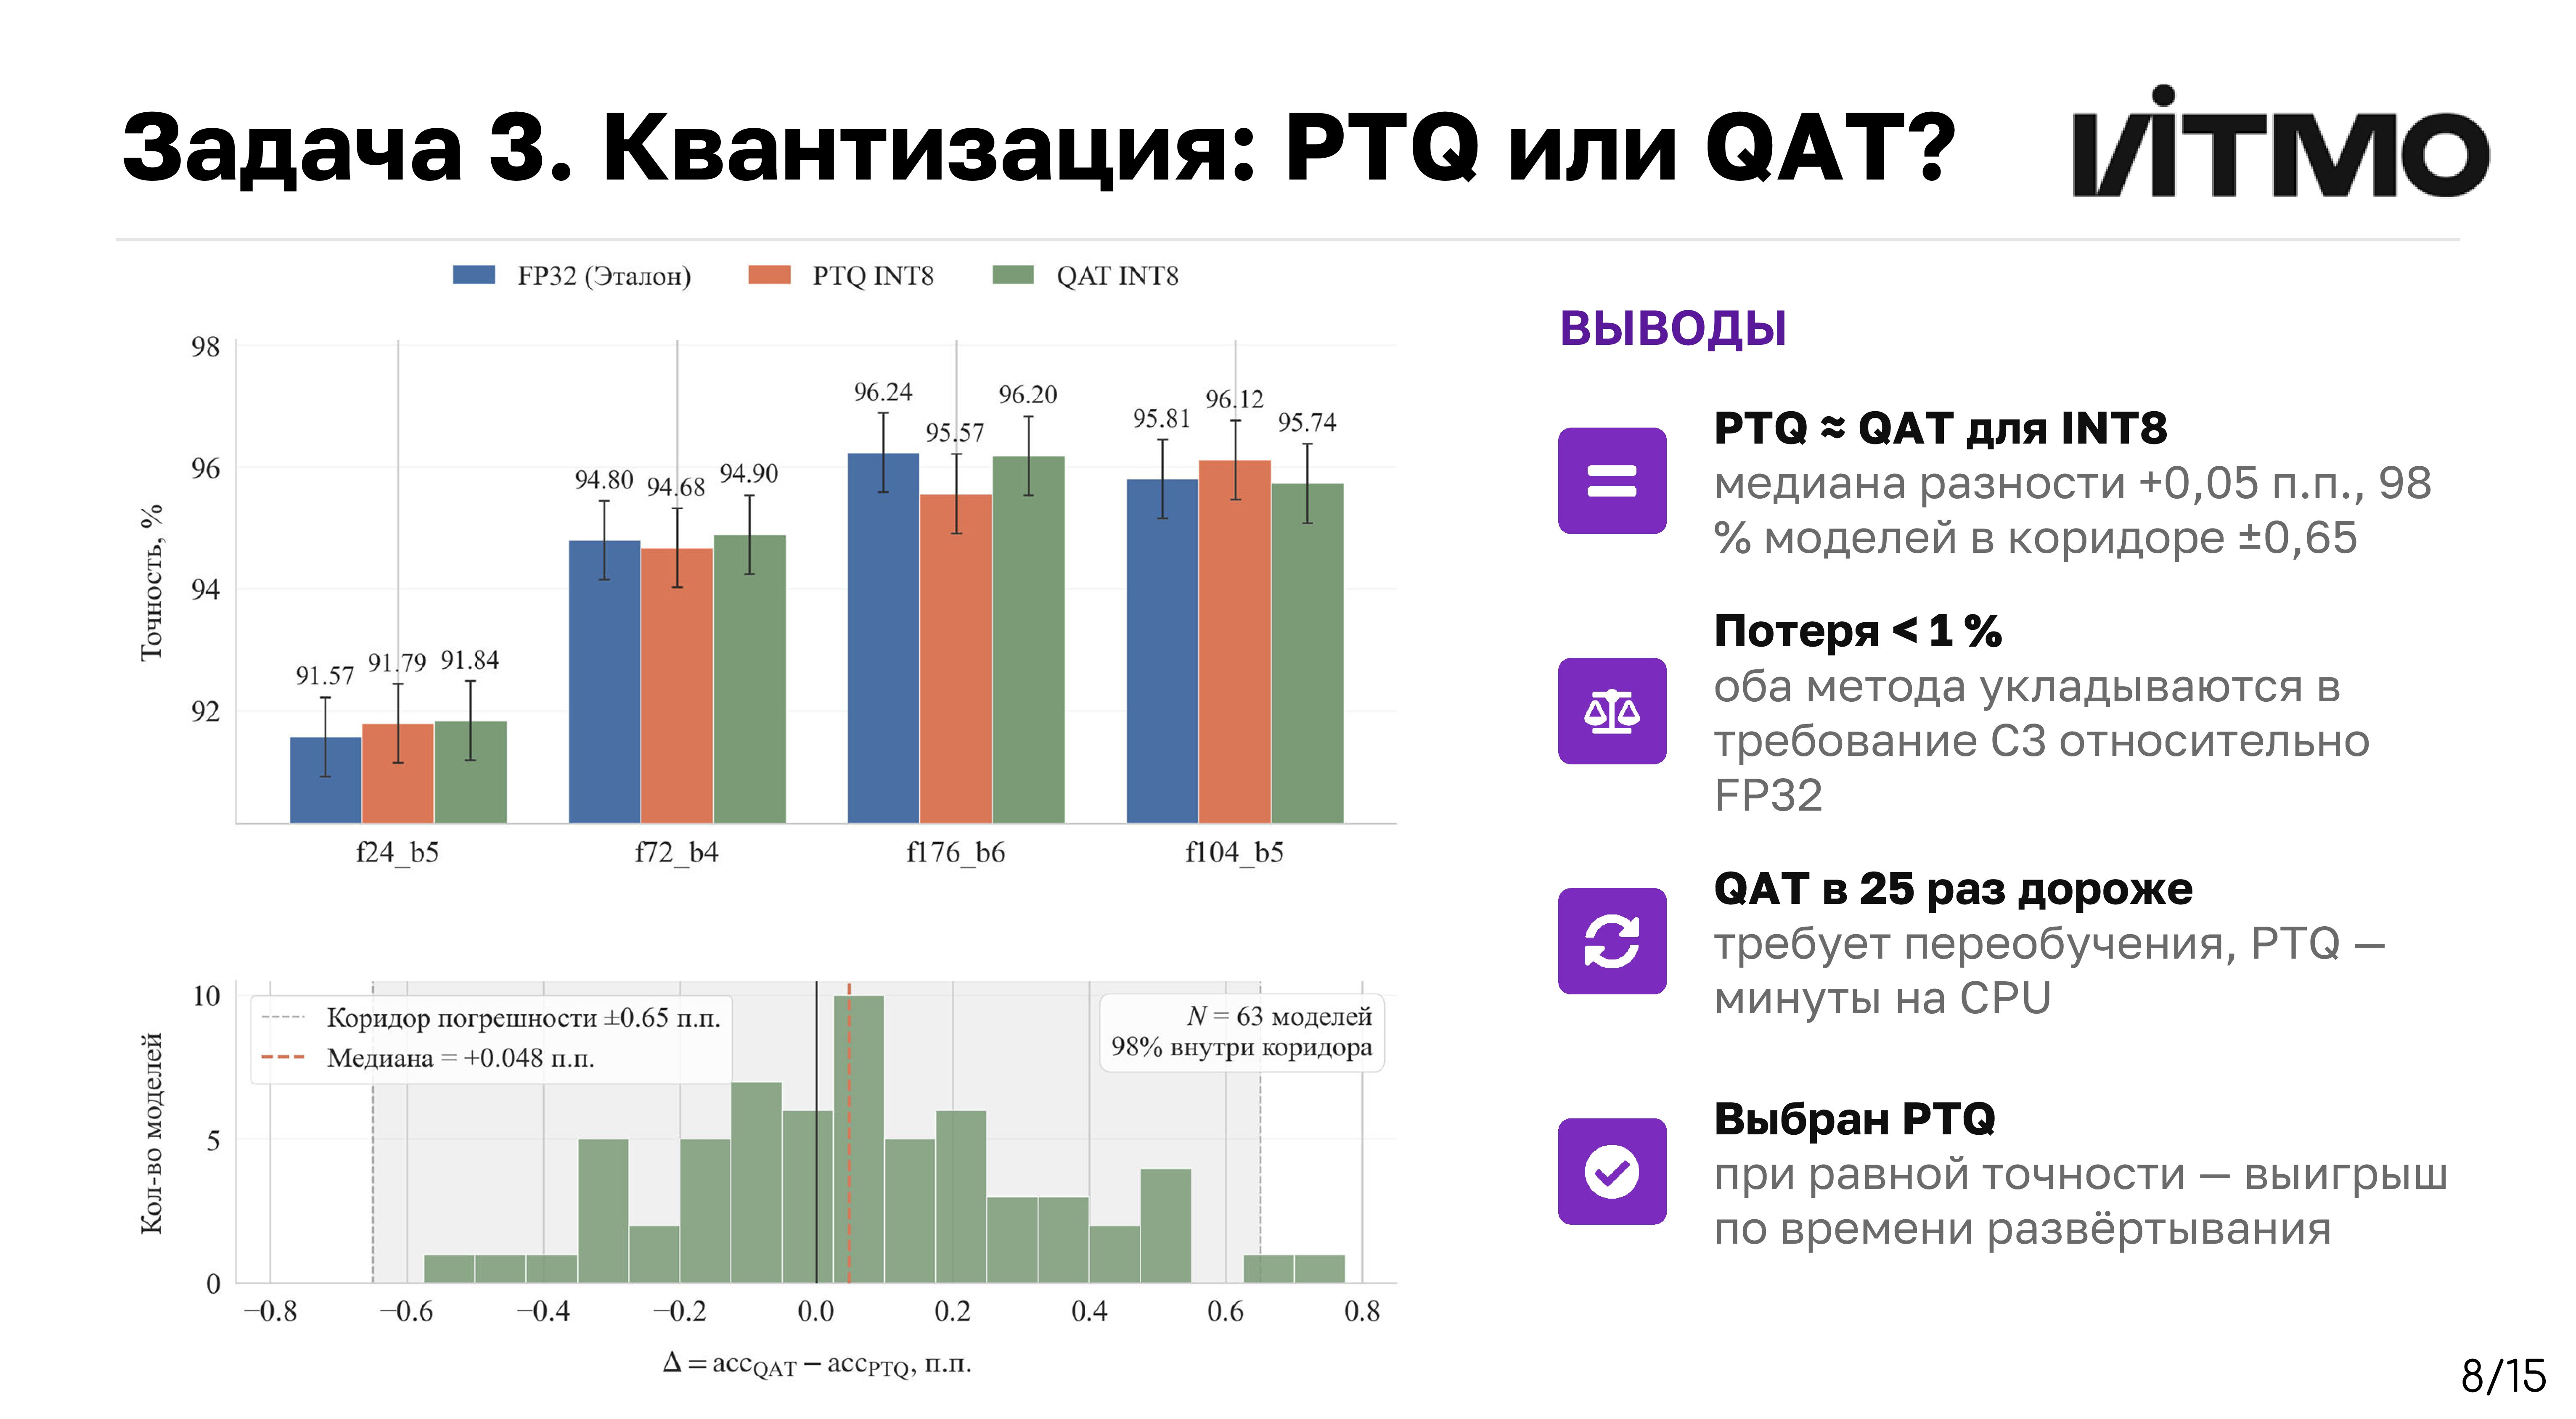
\includegraphics[width=1\textwidth]{docs/ВКР предзащита 2026_08.jpg}
	\caption{Слайд сравнения методов восьмибитной квантизации}
	\label{fig:slide_08}
\end{figure}

\begin{figure}[H]
	\centering
	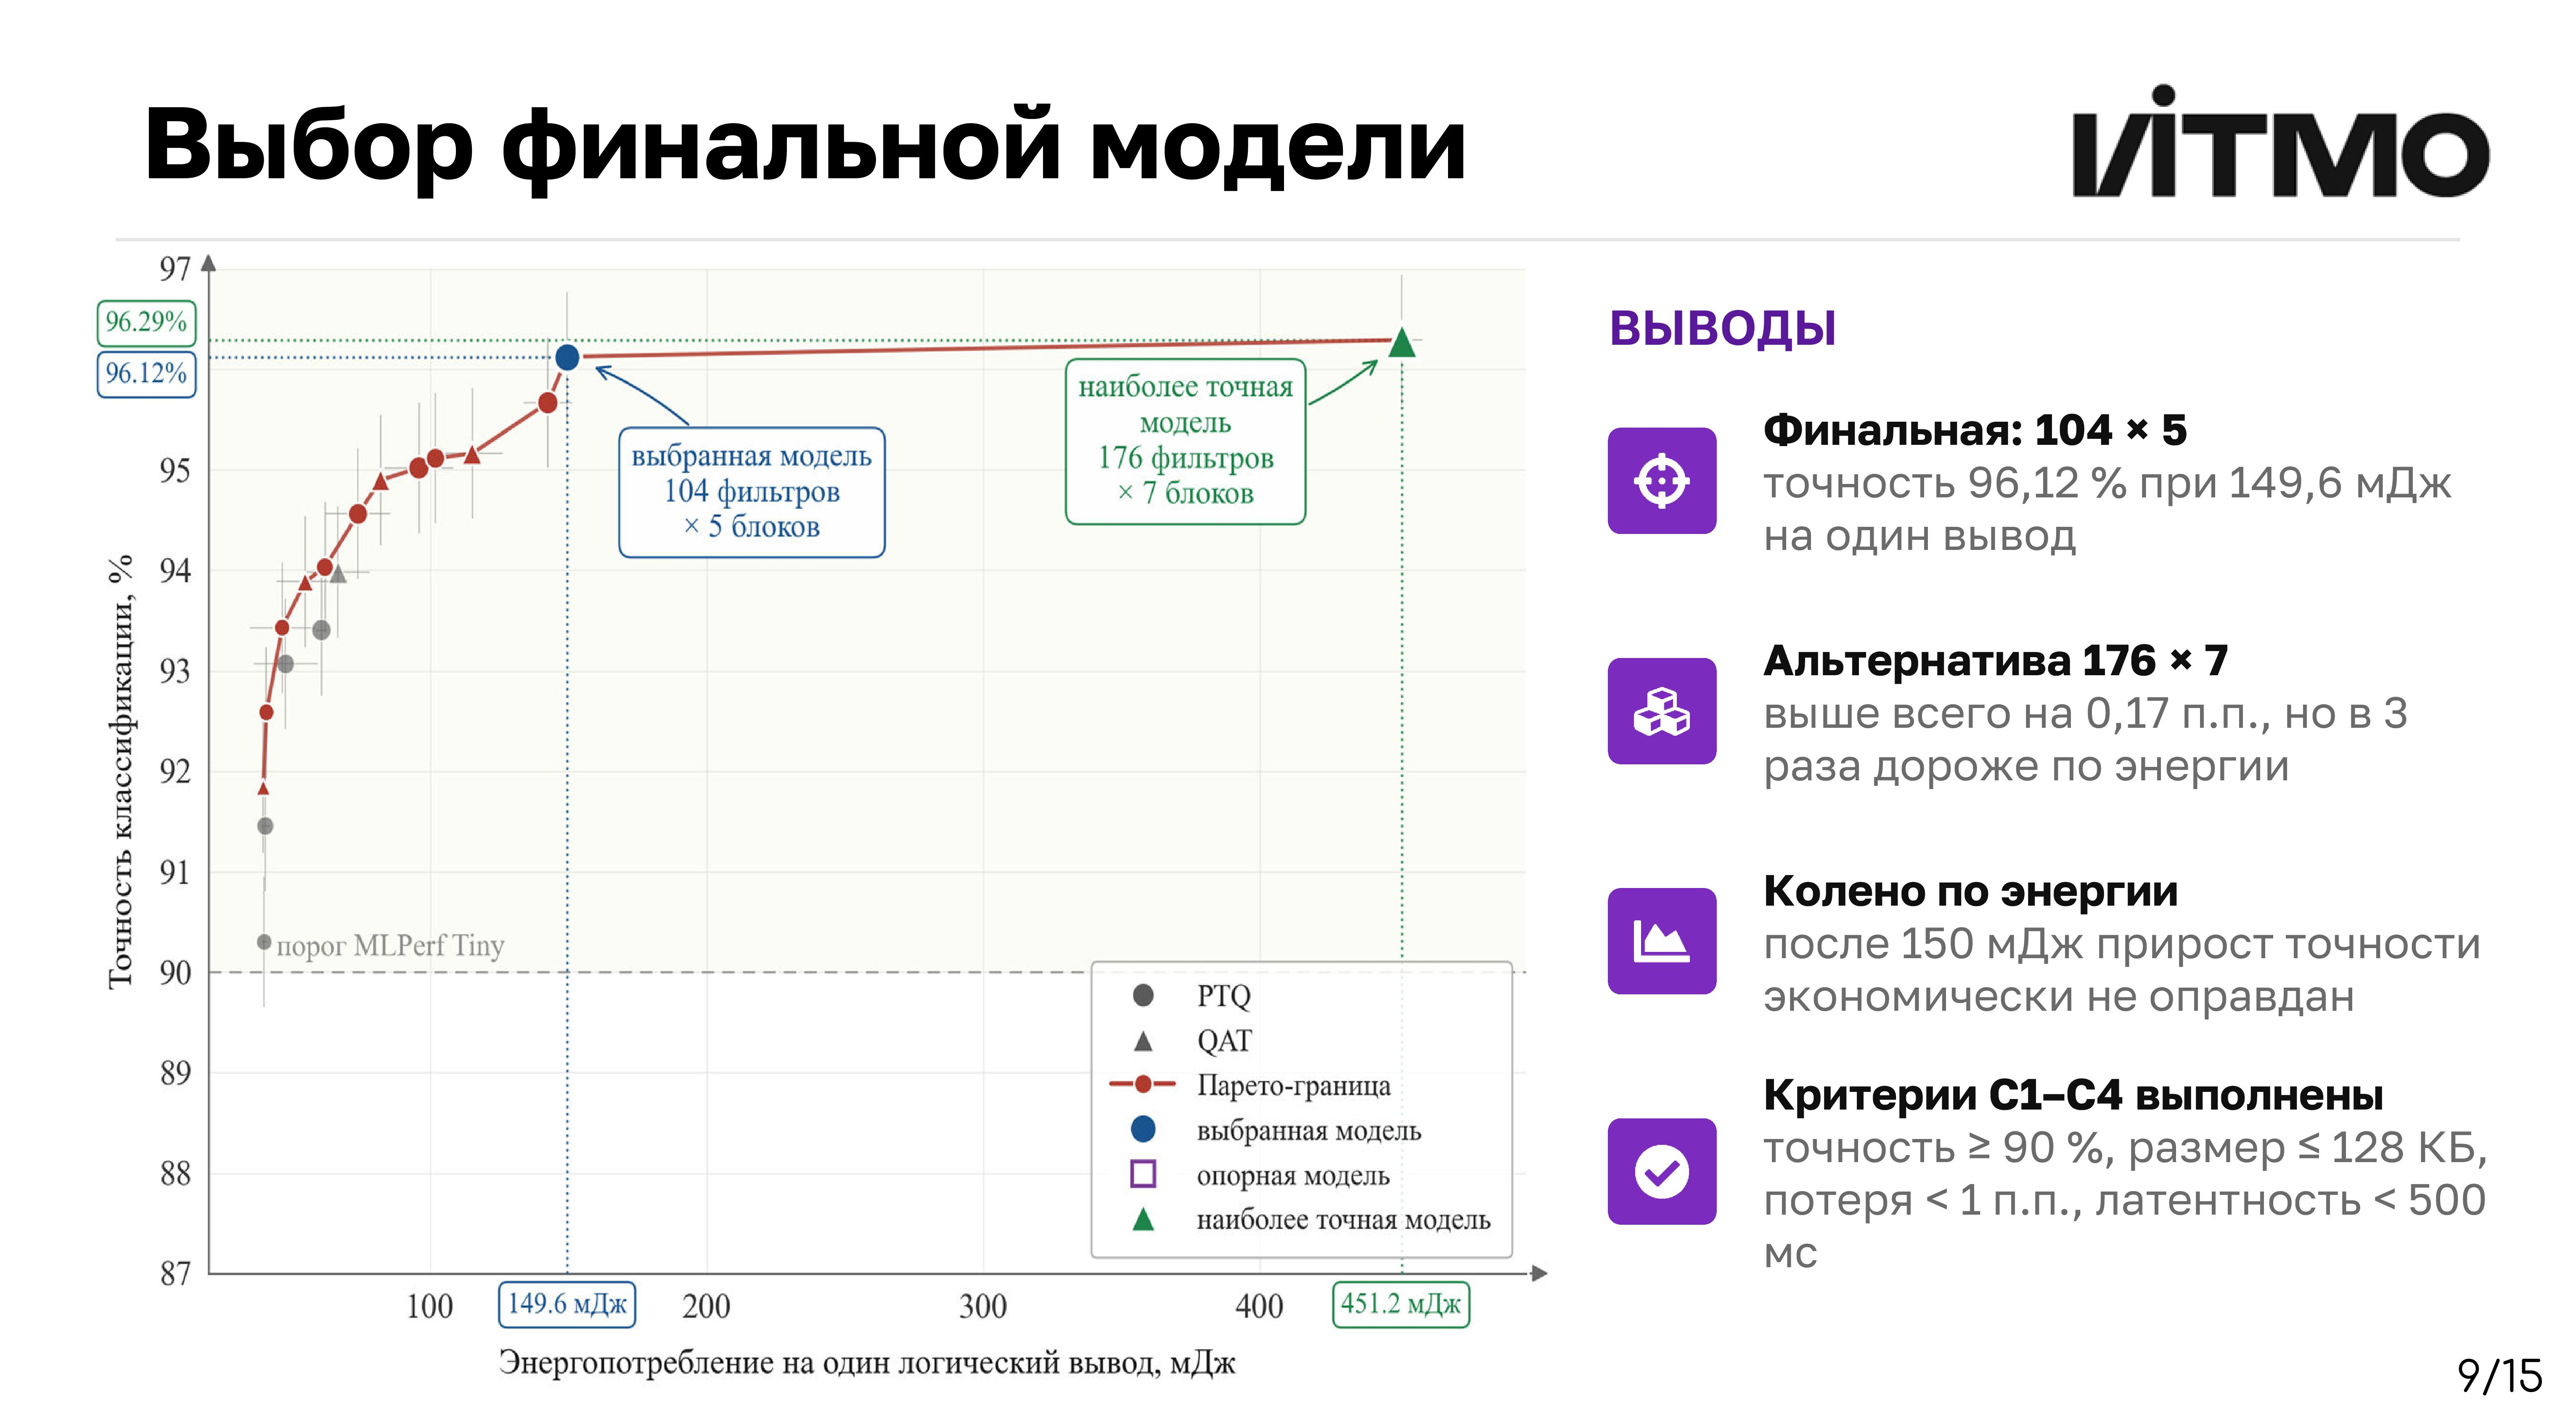
\includegraphics[width=1\textwidth]{docs/ВКР предзащита 2026_09.jpg}
	\caption{Слайд <<Выбор финальной модели>>}
	\label{fig:slide_09}
\end{figure}

\begin{figure}[H]
	\centering
	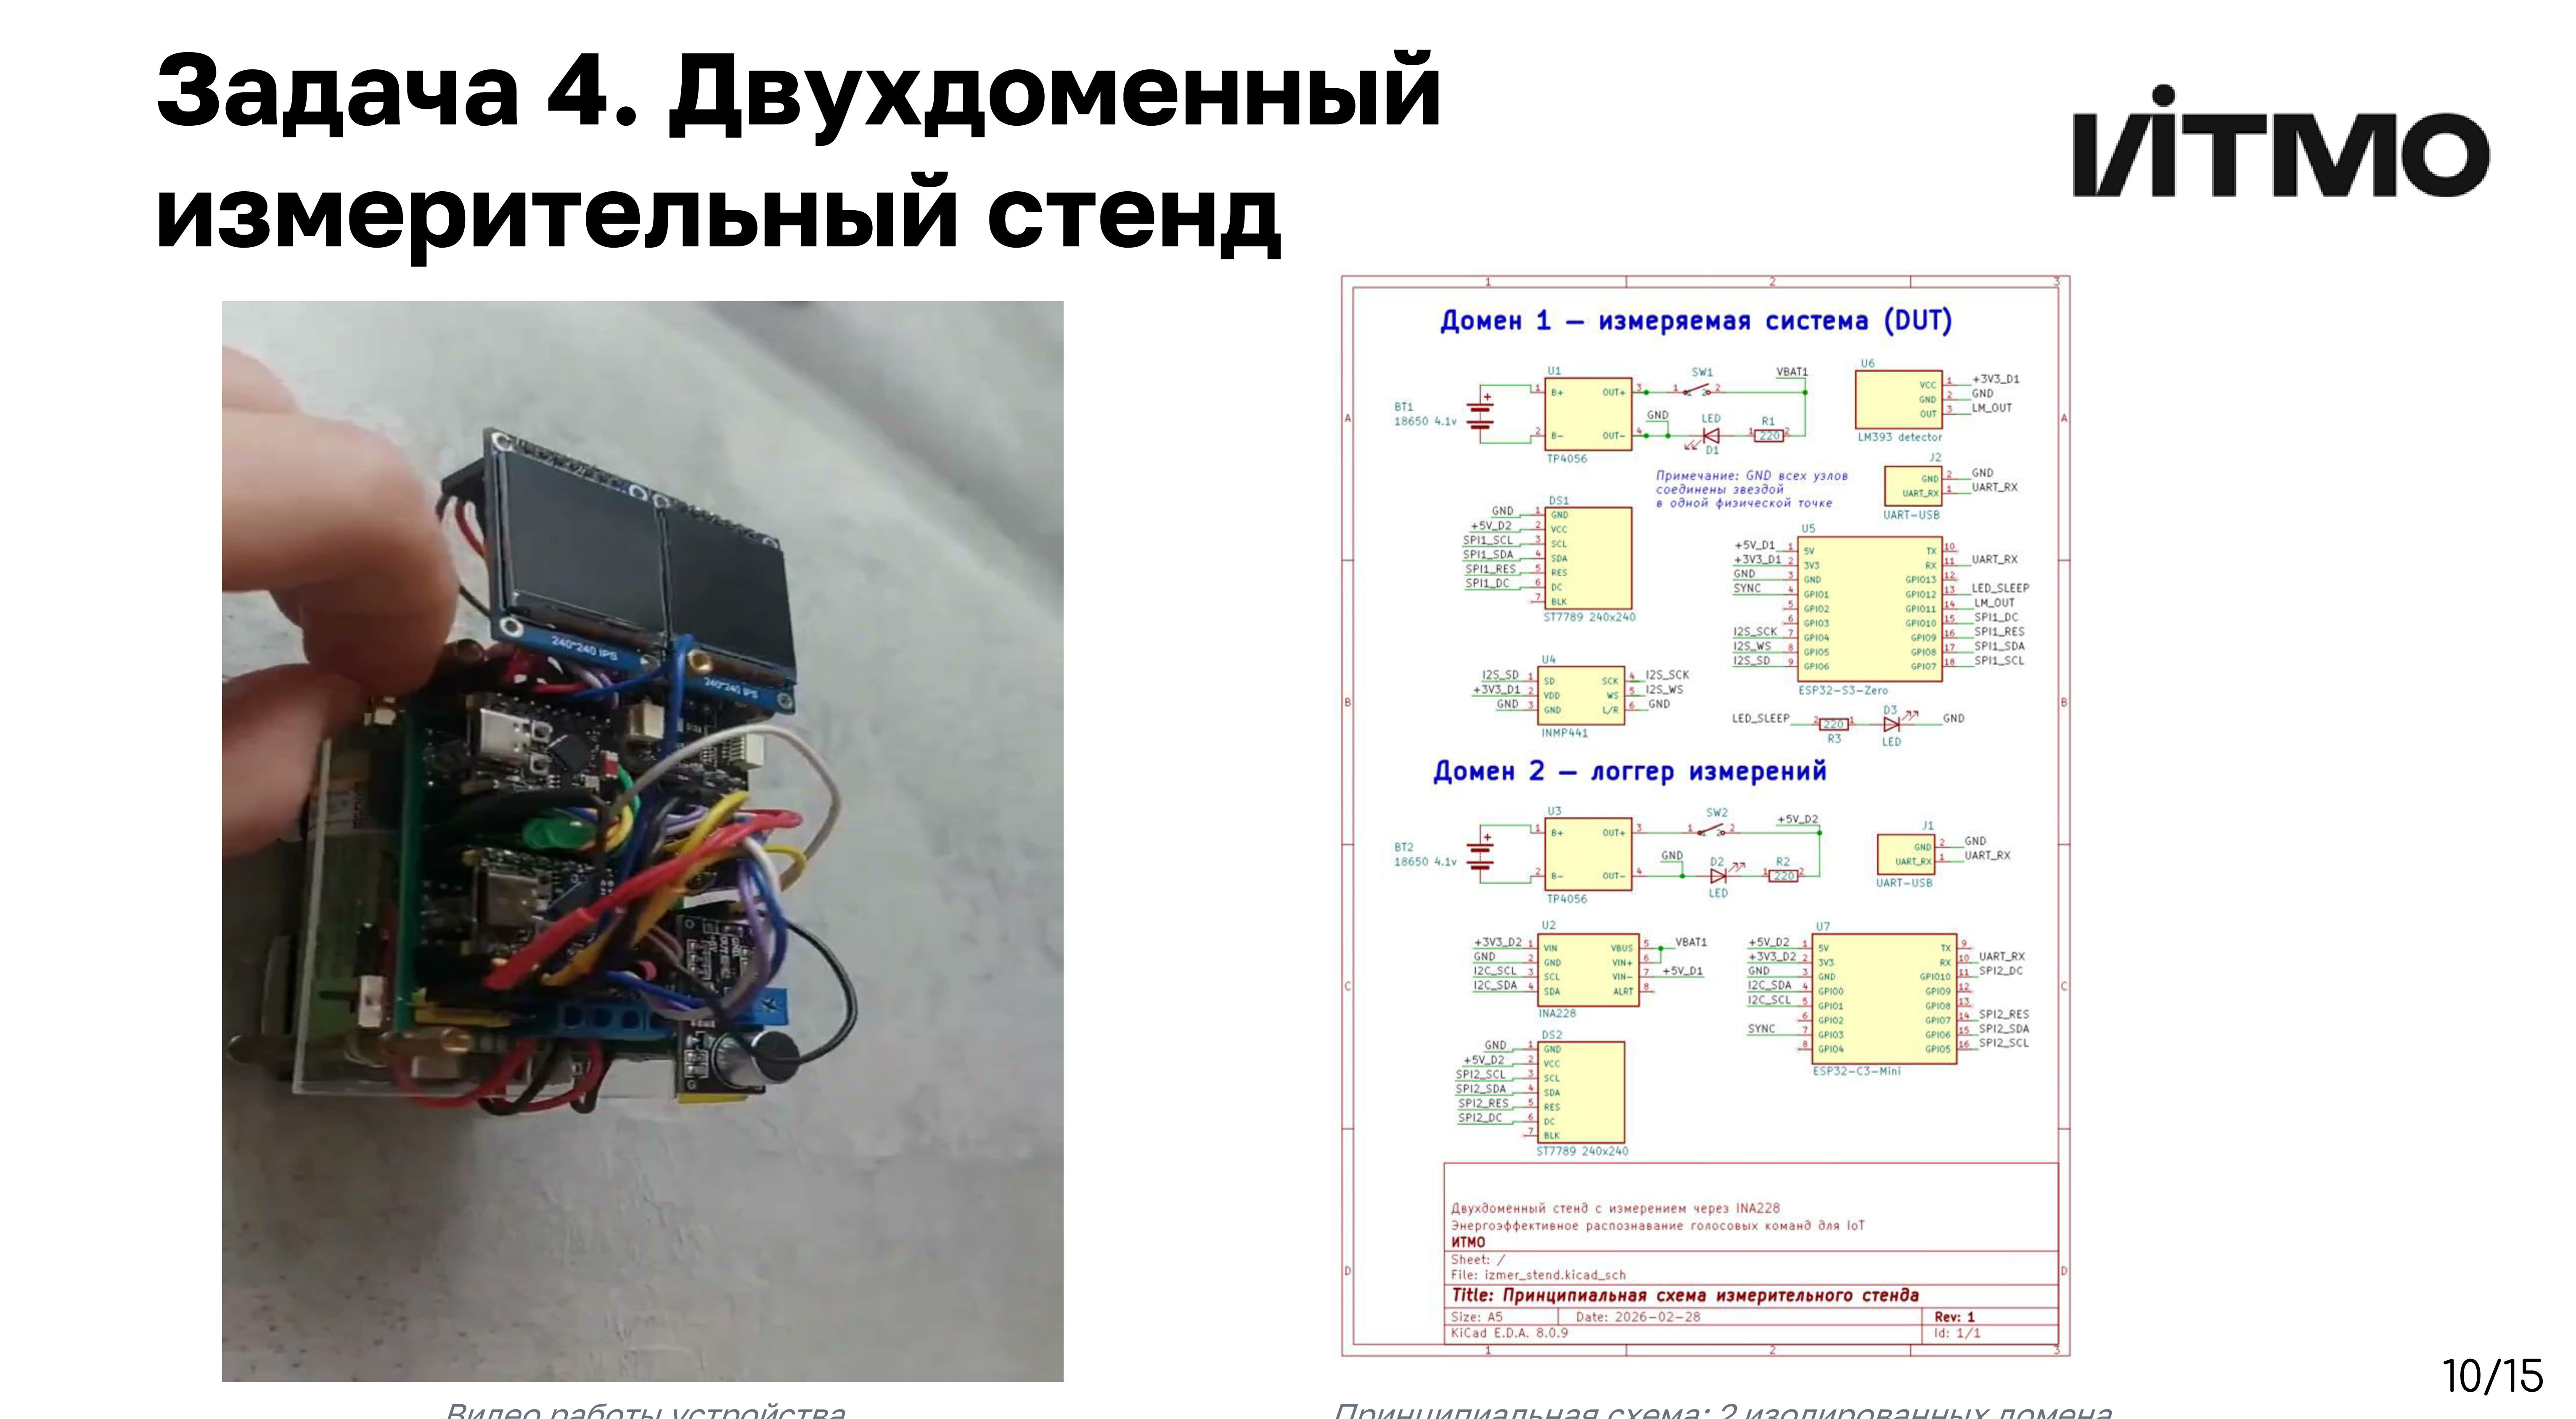
\includegraphics[width=1\textwidth]{docs/ВКР предзащита 2026_10.jpg}
	\caption{Слайд с эксперементальной апробацией на лабораторном стенде}
	\label{fig:slide_10}
\end{figure}

\begin{figure}[H]
	\centering
	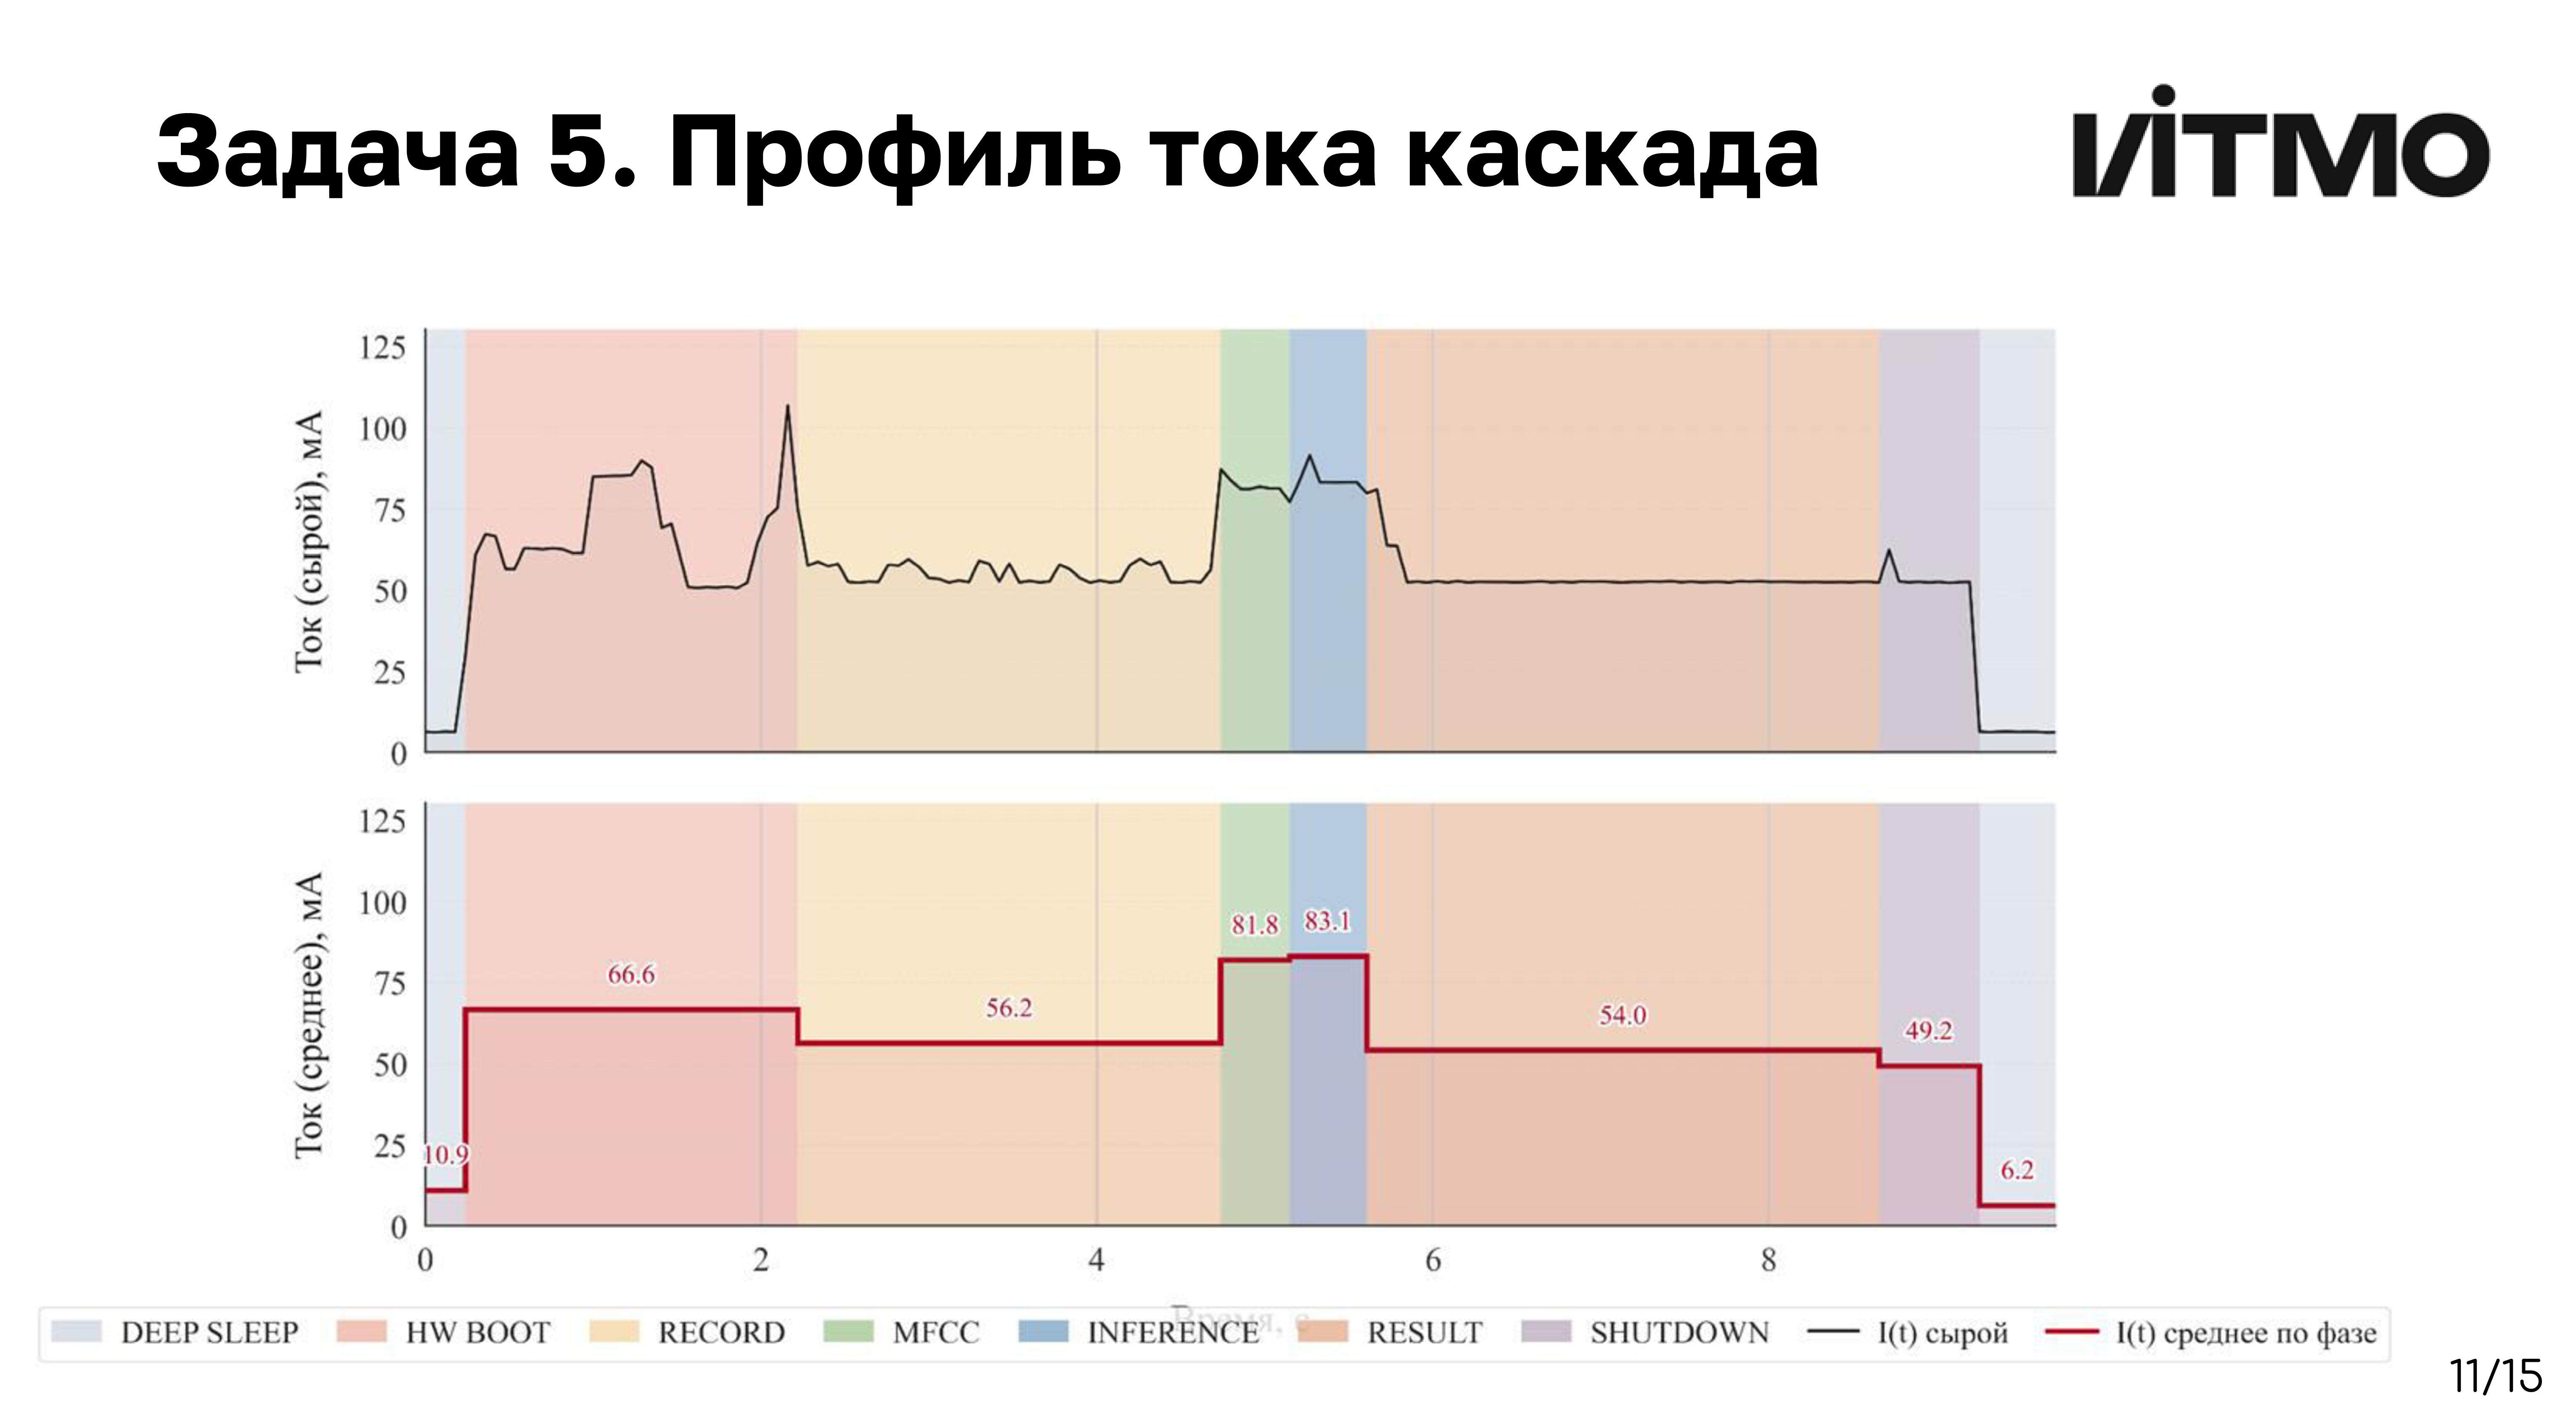
\includegraphics[width=1\textwidth]{docs/ВКР предзащита 2026_11.jpg}
	\caption{Слайд <<Профиль тока каскада>>}
	\label{fig:slide_11}
\end{figure}

\begin{figure}[H]
	\centering
	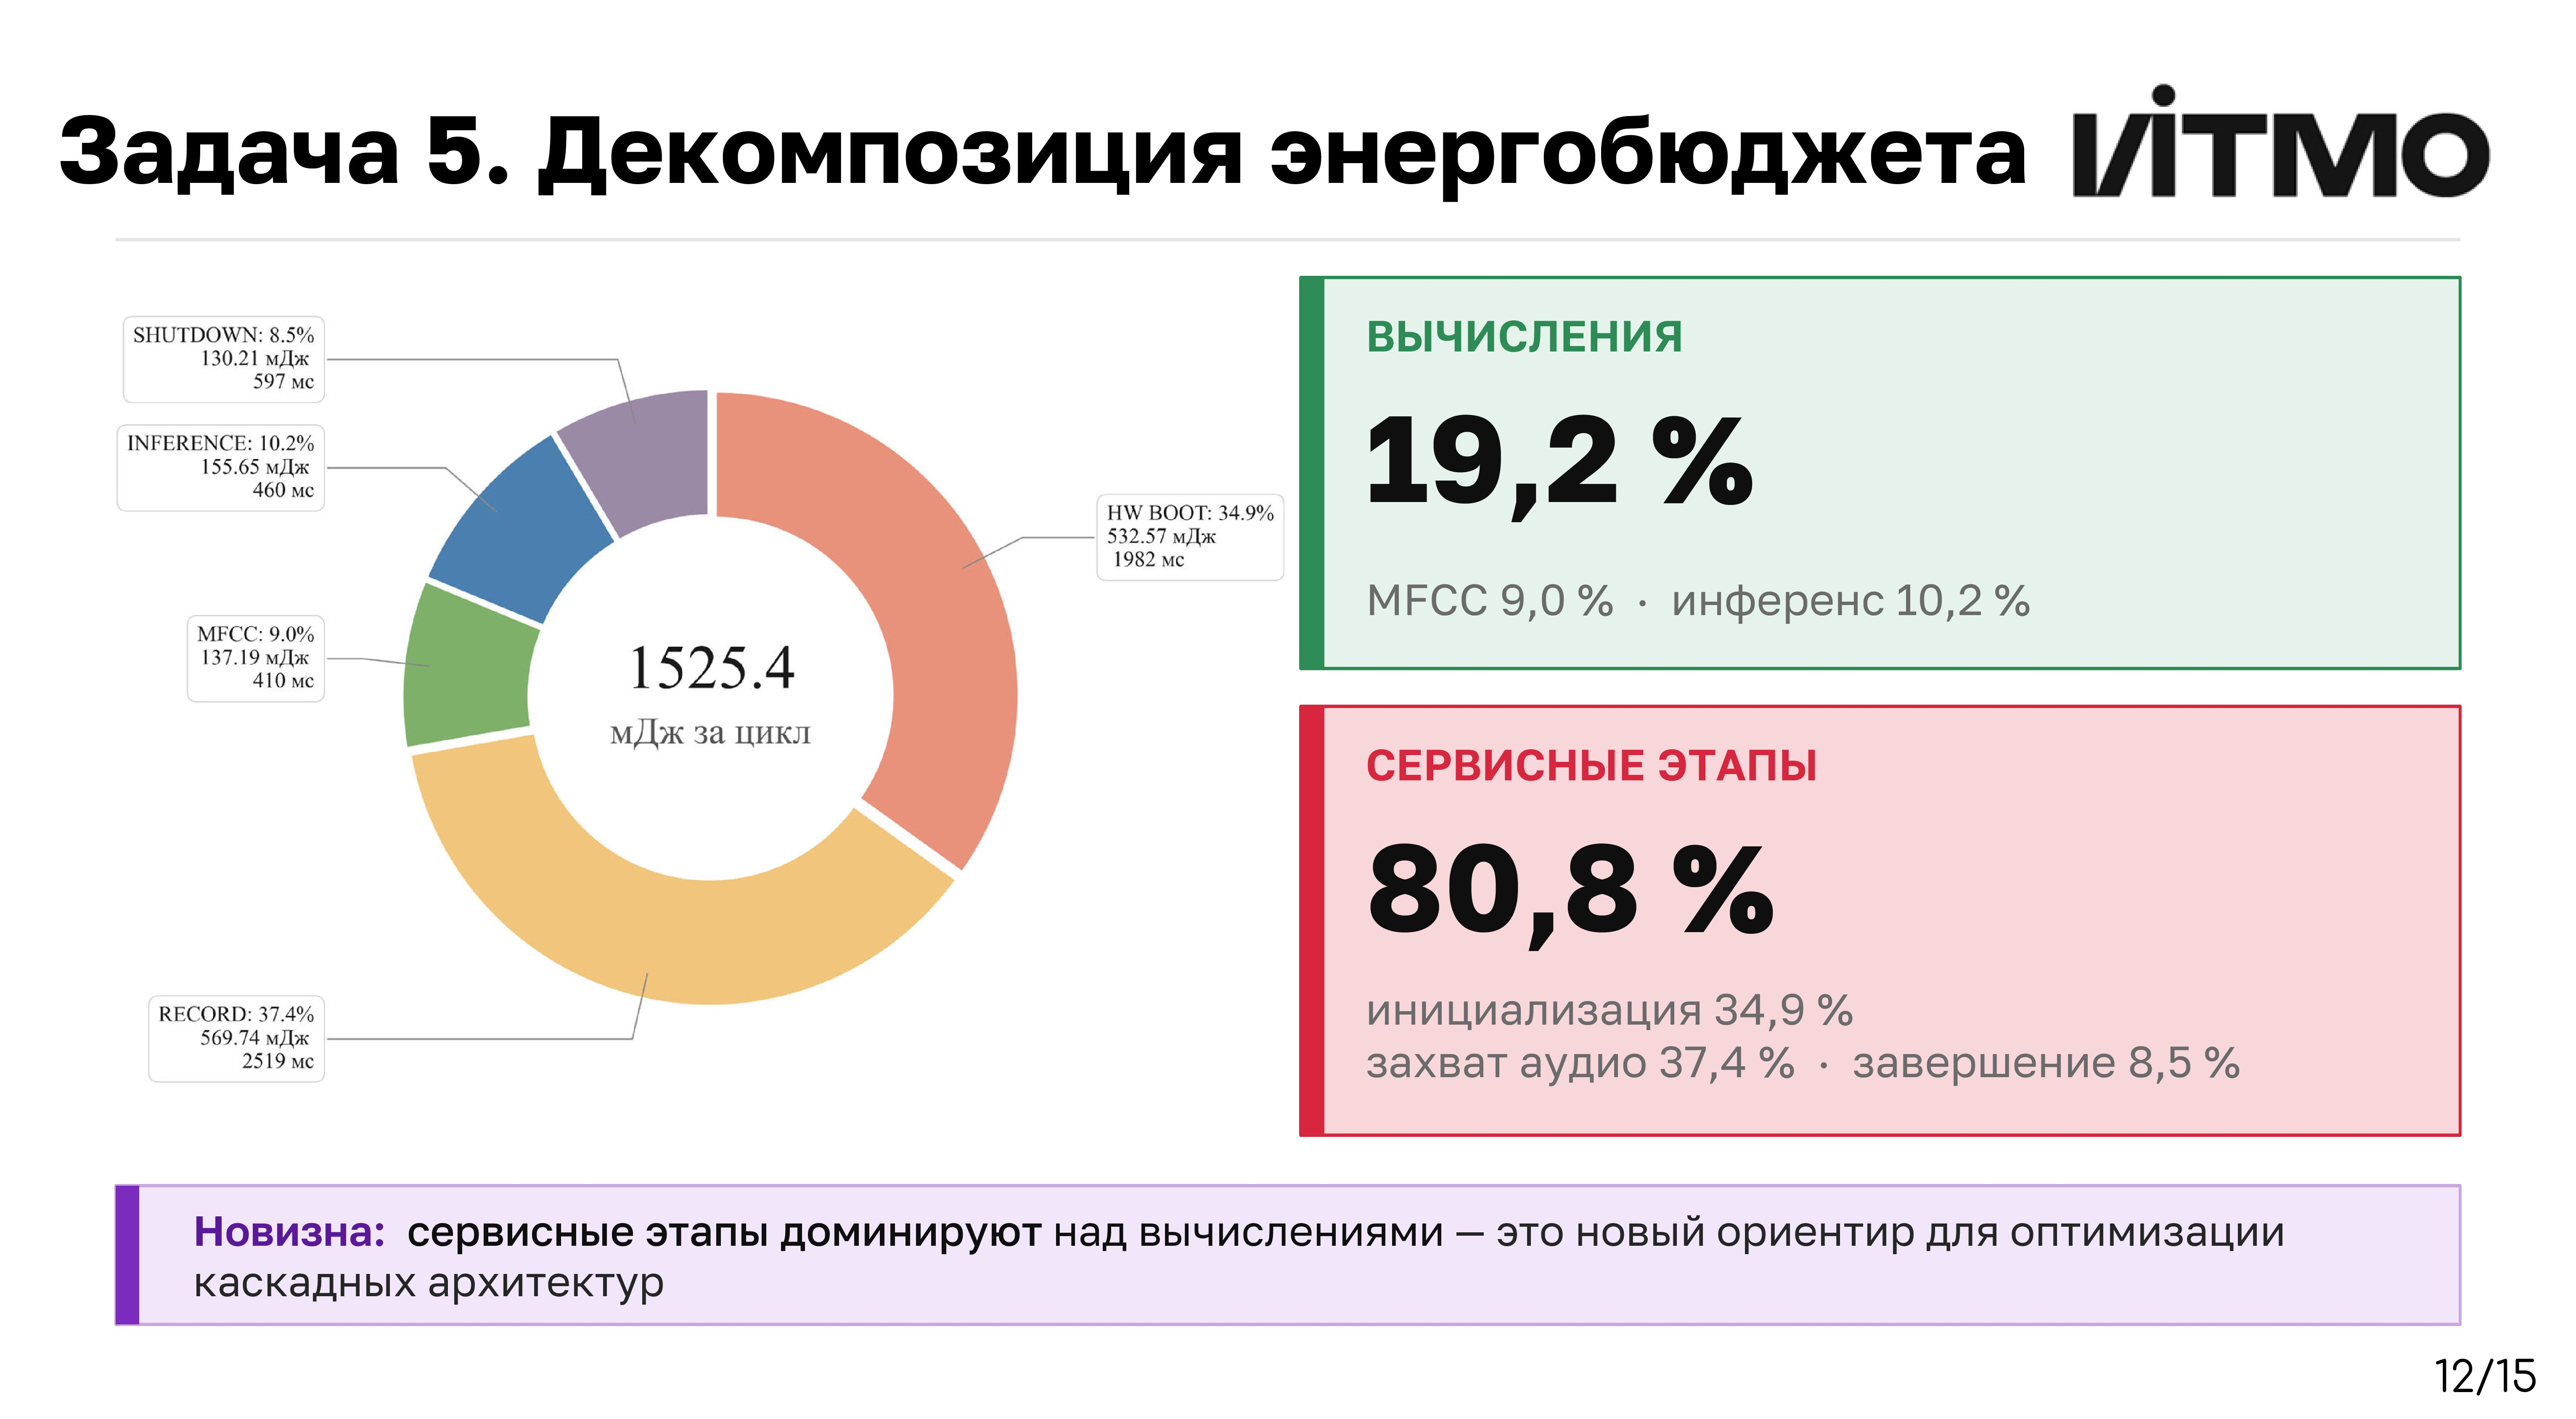
\includegraphics[width=1\textwidth]{docs/ВКР предзащита 2026_12.jpg}
	\caption{Слайд <<Декомпозиция энергобюджета>>}
	\label{fig:slide_12}
\end{figure}

\begin{figure}[H]
	\centering
	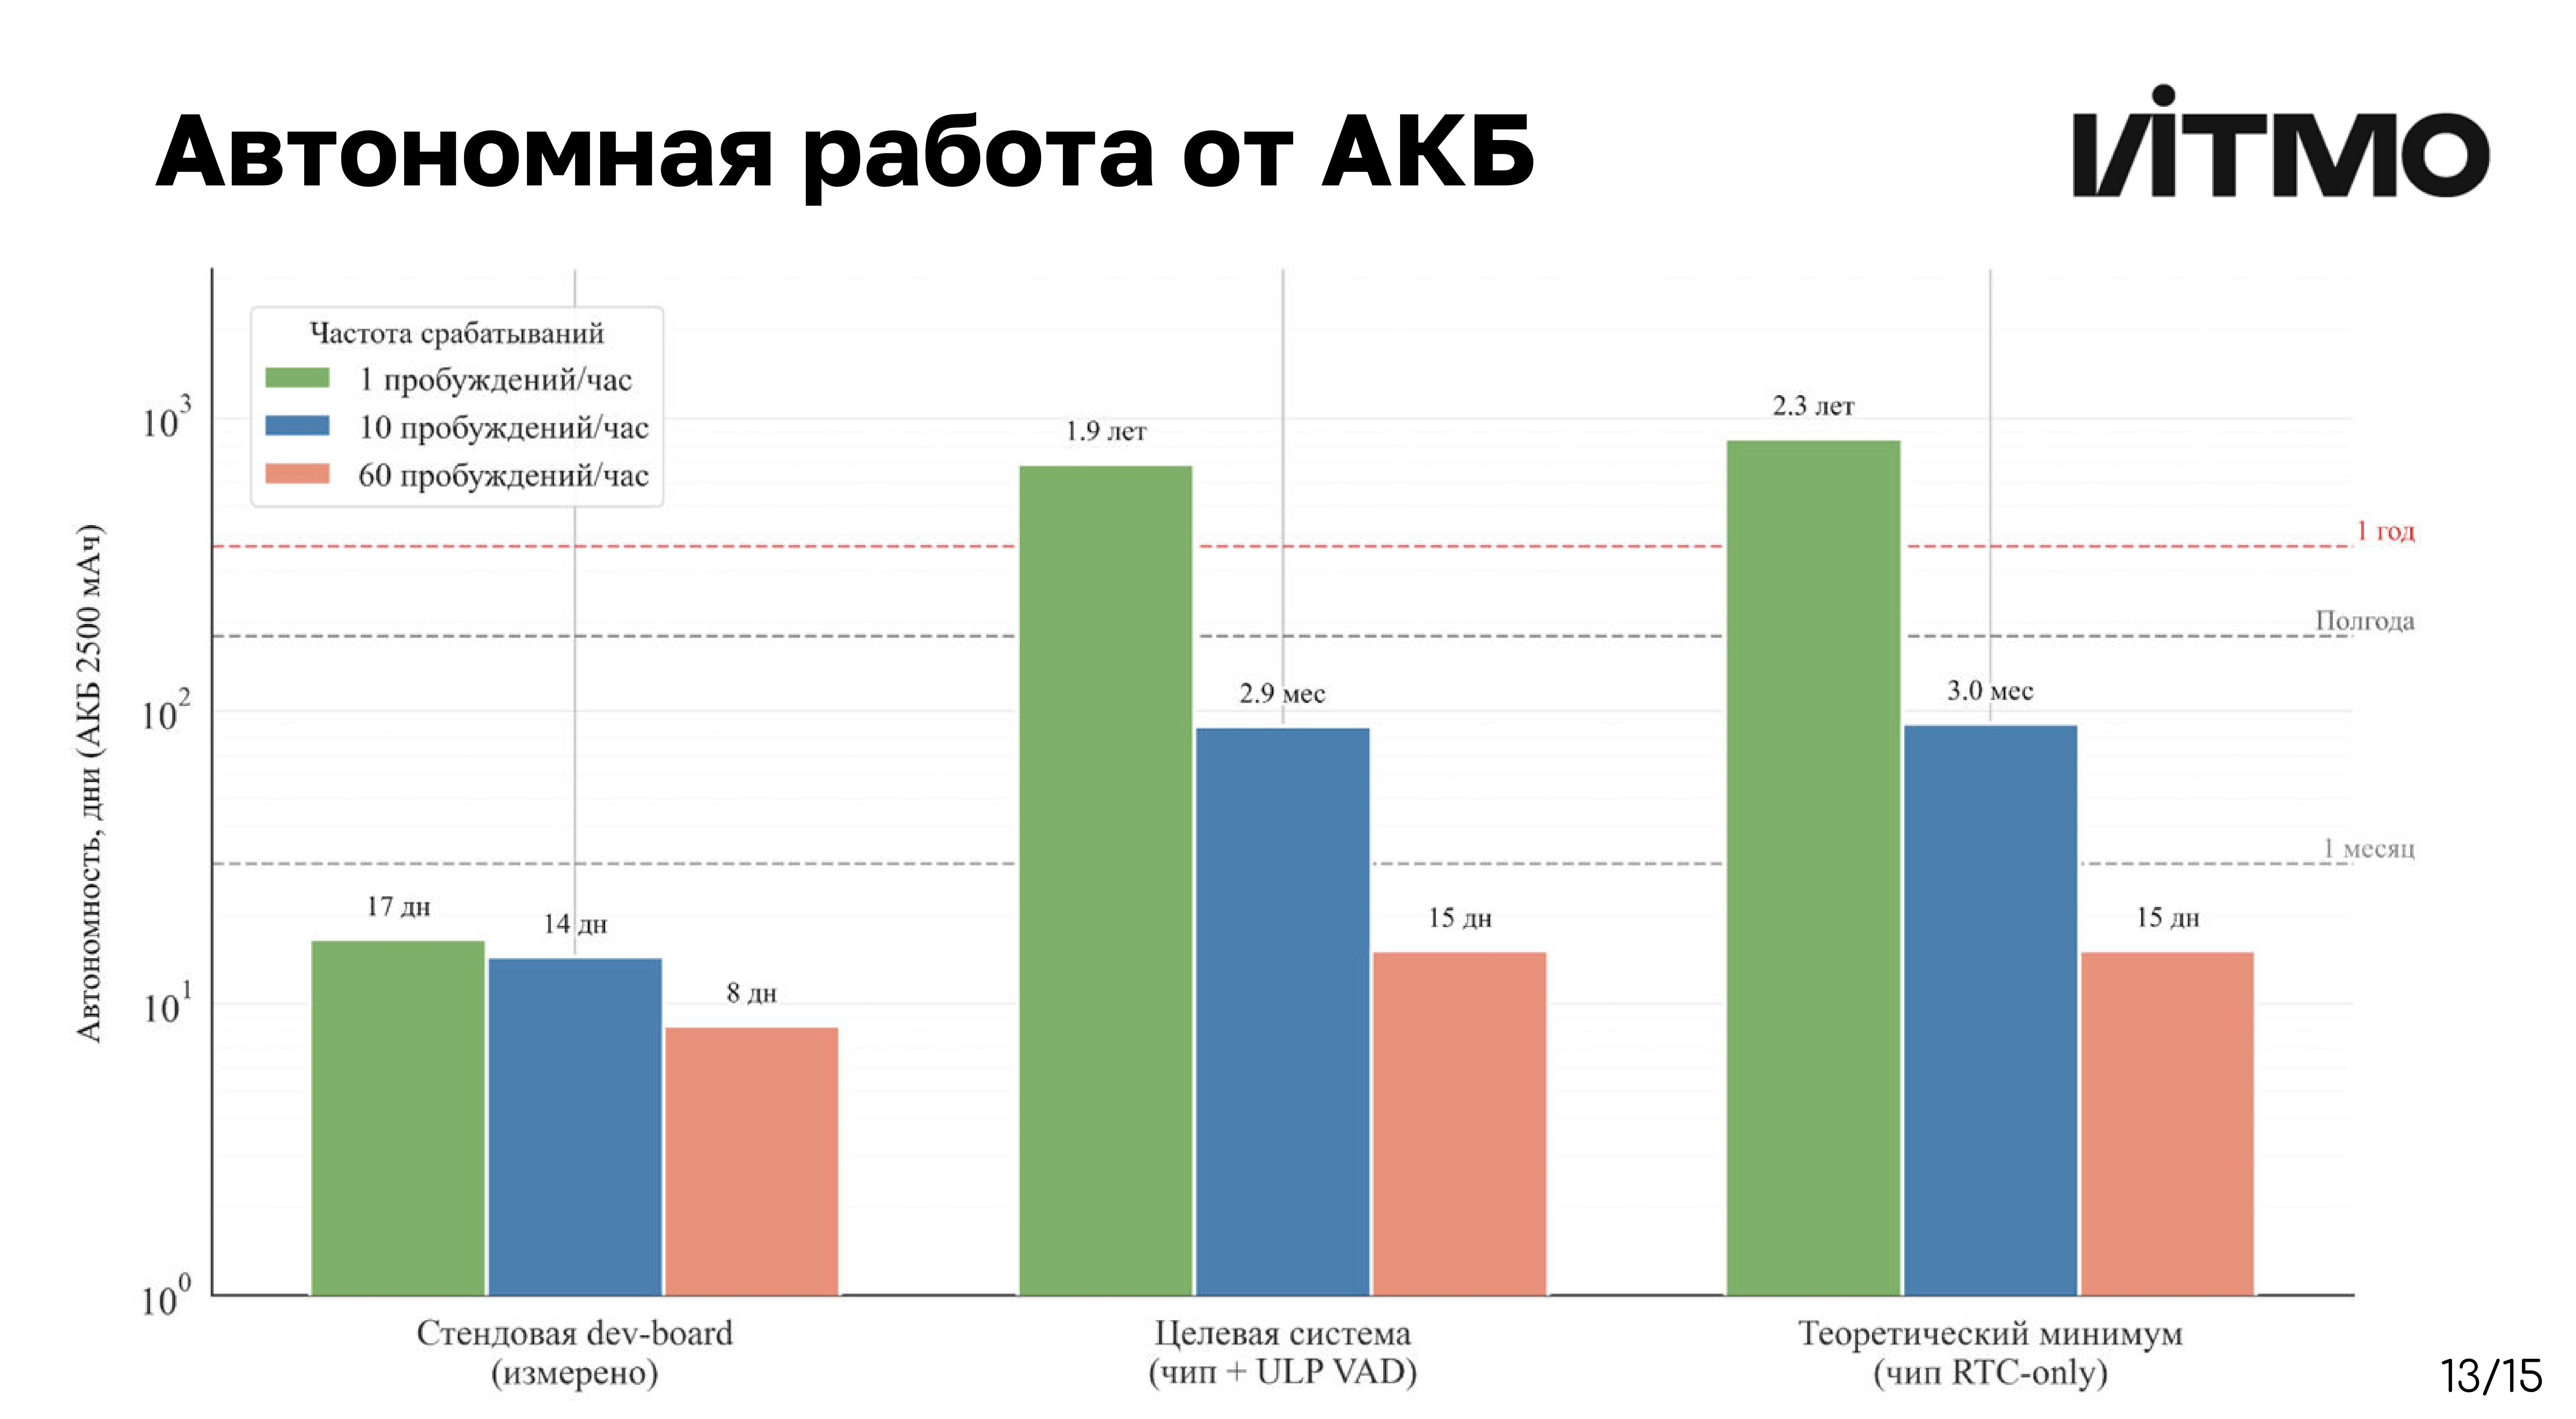
\includegraphics[width=1\textwidth]{docs/ВКР предзащита 2026_13.jpg}
	\caption{Слайд <<Автономная работа от АКБ>>}
	\label{fig:slide_13}
\end{figure}

\begin{figure}[H]
	\centering
	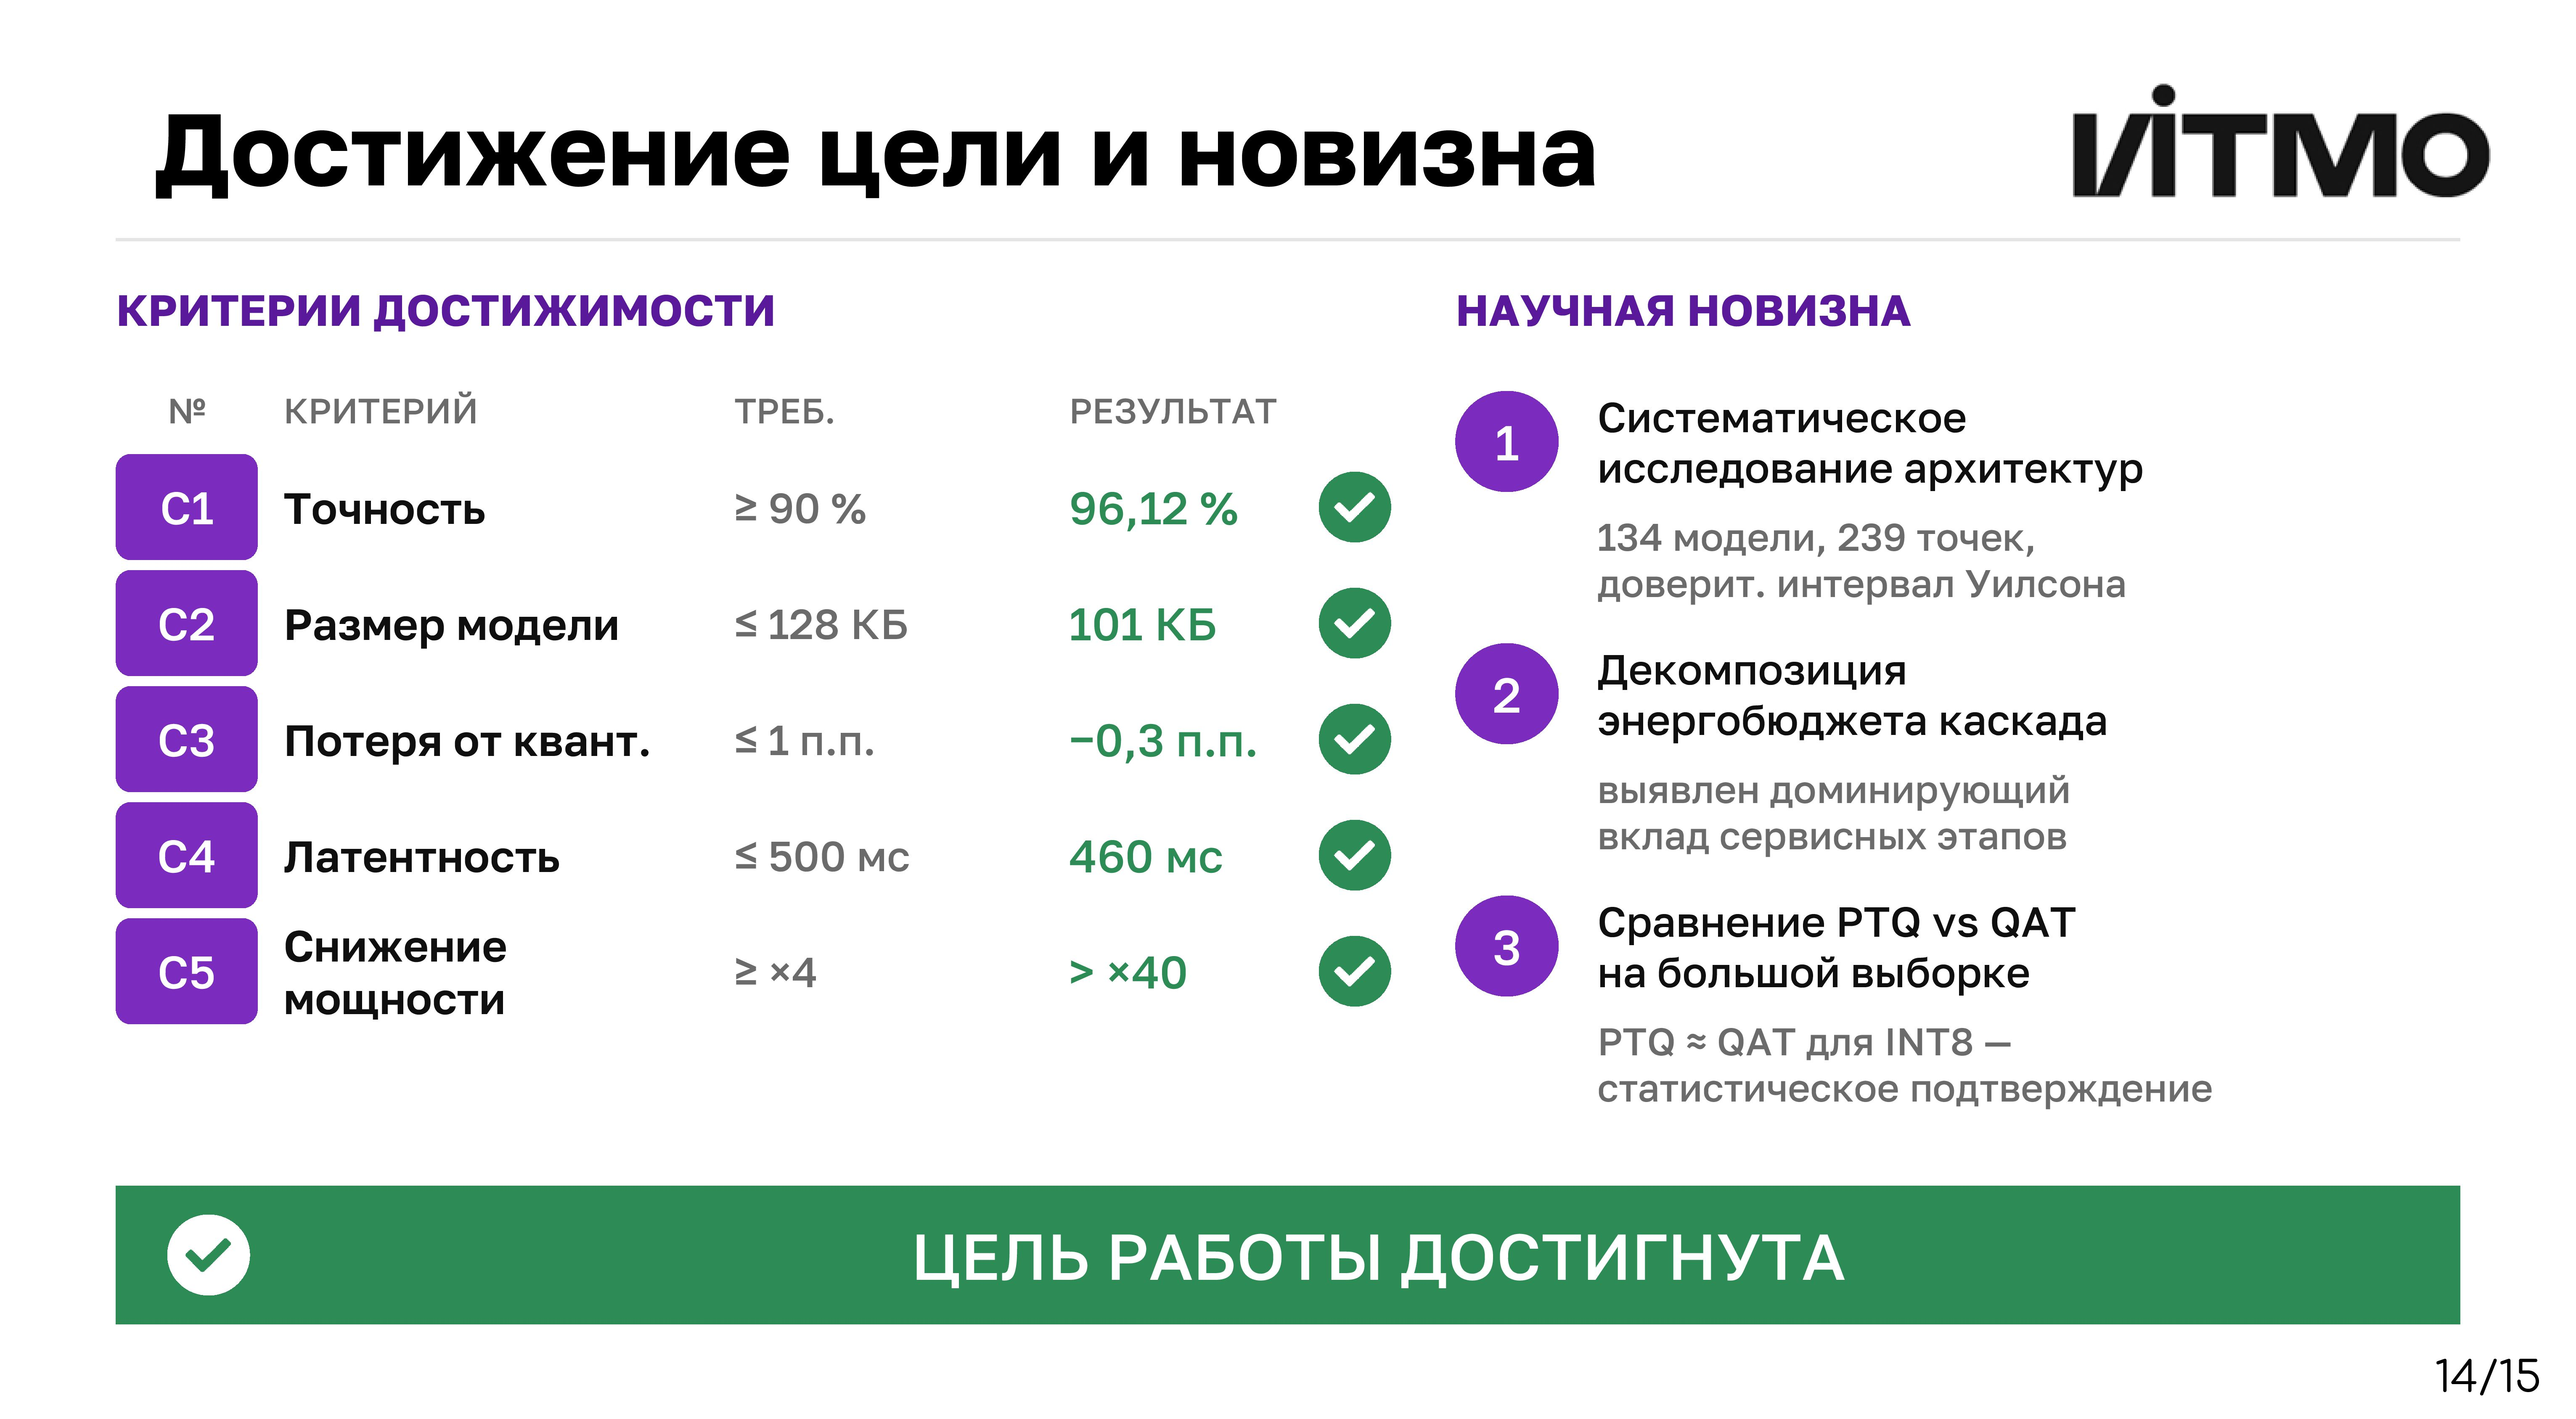
\includegraphics[width=1\textwidth]{docs/ВКР предзащита 2026_14.jpg}
	\caption{Слайд <<Достижение цели и новизна>>}
	\label{fig:slide_14}
\end{figure}

\begin{figure}[H]
	\centering
	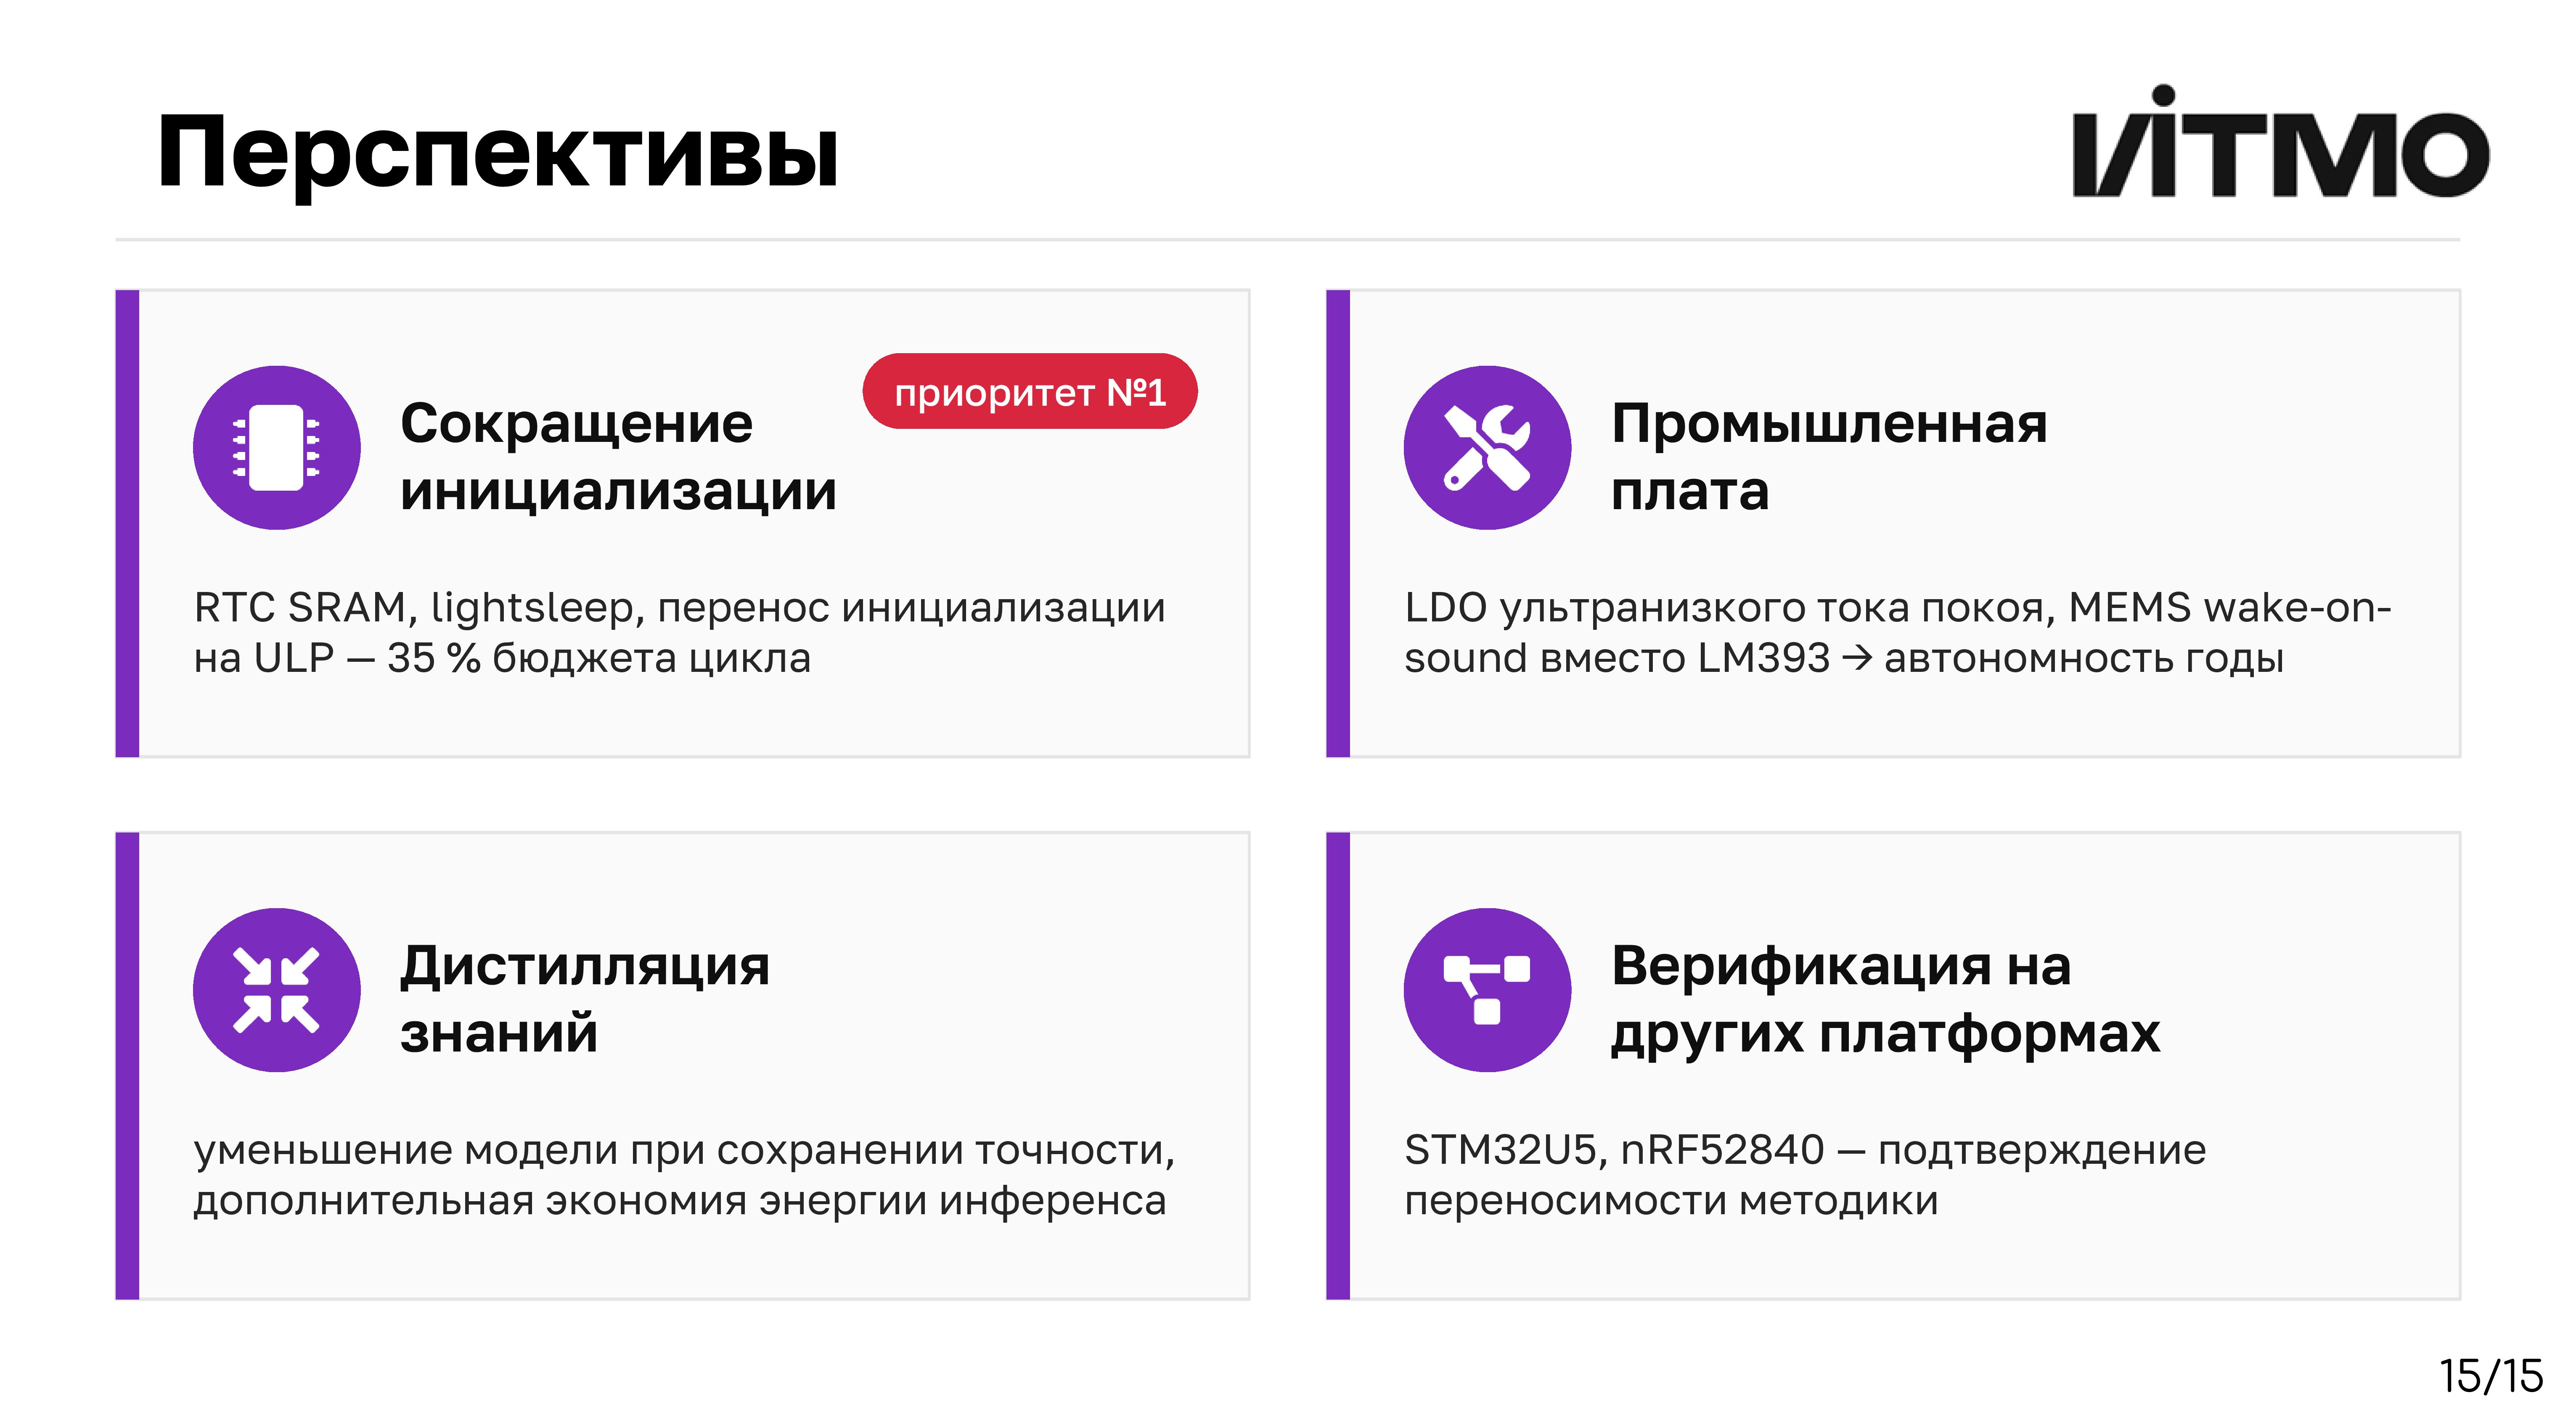
\includegraphics[width=1\textwidth]{docs/ВКР предзащита 2026_15.jpg}
	\caption{Слайд <<Перспективы>>}
	\label{fig:slide_15}
\end{figure}

\begin{figure}[H]
	\centering
	
\includegraphics[width=1\textwidth]{docs/ВКР предзащита 2026_16.jpg}
	\caption{Слайд <<Спасибо за внимание>>}
	\label{fig:slide_15}
\end{figure}

% ----- ПРИЛОЖЕНИЕ В -----
\appsection{Скриншот выступления на предзащите ВКР}
\label{app:predefense_screenshot}

\begin{figure}[H]
	\centering
	
\includegraphics[width=1\textwidth]{docs/predefense_screenshot.png}
	\caption{Скриншот выступления на предзащите ВКР из раздела <<Артефакты>> в Контур Толк}
	\label{fig:predefense_screenshot}
\end{figure}

% ----- ПРИЛОЖЕНИЕ Г -----
\appsection{Исправленный по итогам предзащиты слайд экспериментальной апробации}
\label{app:fixed_slide}

\begin{figure}[H]
	\centering
	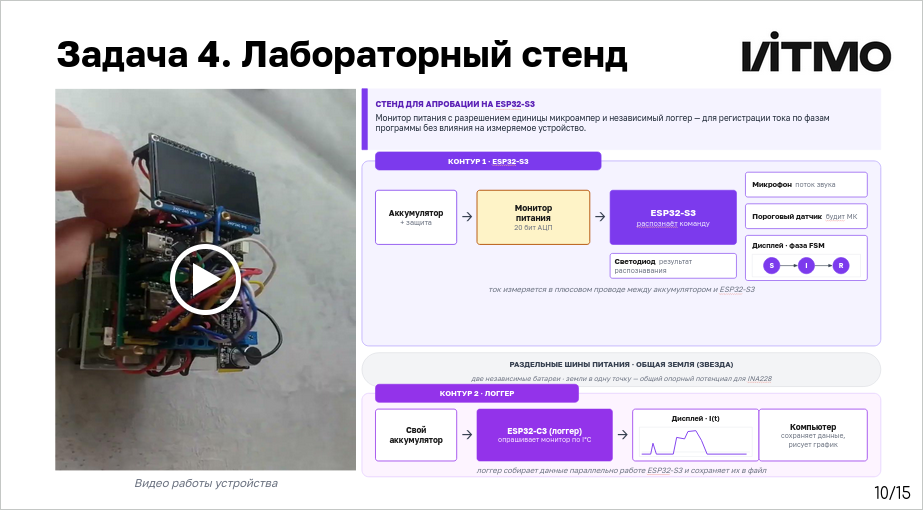
\includegraphics[width=1\textwidth]{docs/fixed_slide.png}
	\caption{Слайд с экспериментальной апробацией, исправленный по итогам предзащиты}
	\label{fig:fixed_slide_img}
\end{figure}
